% !TeX encoding = UTF-8
\chapterimage{chap34.jpg}
\chapter{August}
\section{Week \Rmnum{1}}
\hl{\textbf{\textit{August 1}}}

1. 设函数$f(x)$在$x=x_{0}$的某个邻域内有定义,下列命题中正确的个数:  
\begin{itemize}
	\item \hl{A}. 若$f'(x_{0})$存在,则$f(x)$在$x=x_{0}$处连续
	\item \hl{B}. 若$f'_{-}(x_{0})$和$f'_{+}(x_{0})$都存在,则$f(x)$在$x=x_{0}$处连续
	\item C. 若$\lim\limits_{x\rightarrow x_{0}^{-}}f'(x)$,$\lim\limits_{x\rightarrow x_{0}^{+}}f'(x)$都存在,则$f(x)$在$x=x_{0}$处连续
	\item D. 若$\lim\limits_{x\rightarrow x_{0}}f'(x)$存在,则$f(x)$在$x=x_{0}$处连续
\end{itemize}
\myspace{1}
\begin{solution}

	$A$. 导函数存在,原函数连续,正确
	
	$B$. 左右导数存在,我们得到:  
	$$\left\lbrace
	\begin{array}{l}
		\lim\limits_{x\rightarrow x_{0}^{+}}\dfrac{f(x)-f(x_{0})}{x-x_{0}}=A\\
		\lim\limits_{x\rightarrow x_{0}^{-}}\dfrac{f(x)-f(x_{0})}{x-x_{0}}=B
	\end{array}
	\right. \Rightarrow \lim\limits_{x\rightarrow x_{0}}f(x)=f(x_{0})$$
	
	函数$f(x)$在$x=x_{0}$处连续.
	
	$C\text{、}D$ 我们取$f(x)=sign(x)=\left\lbrace
	\begin{array}{l}
		1,\ x>0\\
		0,\ x=0\\
		-1,\ x<0
	\end{array}
	\right. $,此时$\lim\limits_{x\rightarrow 0^{-}}f'(x)=\lim\limits_{x\rightarrow 0^{-}}f'(x)=0$,函数在$x=x_{0}$处间断.
	
	综上所述,上述命题正确的个数为$2$个.
\end{solution}
\myspace{1}

2. $A$为$3$阶实对称矩阵,特征值为$0,1,1$,且$\alpha_{1}=\left( \begin{matrix}
	1\\a\\0
\end{matrix}\right)$,$\alpha_{2}=\left( \begin{matrix}
	1\\-1\\a
\end{matrix}\right)$是$A$的两个不同的特征向量,若$A(\alpha_{1}+\alpha_{2})=\alpha_{2}$,求矩阵$A$
\myspace{1}
\begin{solution}

	(1). 我们可以得到:  
	
	$\alpha_{1}$是矩阵$A$特征值$0$对应的特征向量;\ $\alpha_{2}$是矩阵$A$特征值$1$对应的特征向量.
	
	(2). 我们知道实对称矩阵不同特征值对应的特征向量是正交的$\Rightarrow \alpha_{1}^{T}\alpha_{2}=0\Rightarrow a=1$
	
	(3). 根据谱分解定理,我们可以得到:  $A=\sum\limits_{i=1}^{3}\lambda_{i}G_{i}$
	
	我们发现矩阵$A-E$更好求,因为矩阵$A-E$的特征值为$-1,0,0$,因此$A-E=-G_{1}=-e_{1}e_{1}^{T}$,我们得到:  
	$$\left\lbrace
	\begin{array}{l}
		A=E-e_{1}e_{1}^{T}\\
		e_{1}=\dfrac{1}{\sqrt{2}}\left( \begin{matrix}
			1\\1\\0
		\end{matrix}\right) 
	\end{array}
	\right. \Rightarrow A=\left[ \begin{matrix}
		\dfrac{1}{2}&-\dfrac{1}{2}&0\\
		-\dfrac{1}{2}&\dfrac{1}{2}&0\\
		0&0&1
	\end{matrix}\right] $$
\end{solution}
\myspace{1}

\hl{\textbf{\textit{August 2}}}

1. 设曲线$y=f(x)$与$y=\sqrt{\dfrac{(1+x^2)\sqrt{x}}{e^{x-1}}}+\arctan\dfrac{x^2-1}{\sqrt{1+x^2}}$在点$(1,\sqrt{2})$处相切,求$\lim\limits_{x\rightarrow1}(f(x)+1-\sqrt{2})^{\frac{1}{\ln x}}$
\myspace{1}
\begin{solution}

	原极限可以化为:  
	\begin{eqnarray*}
		I&=&e^{\lim\limits_{x\rightarrow1}\dfrac{\ln(f(x)+1-\sqrt{2})}{\ln x}}\\
		&=&e^{\lim\limits_{x\rightarrow1}\dfrac{f(x)-\sqrt{2}}{x-1}}\\
		&=&e^{\lim\limits_{x\rightarrow1}f'(x)}
	\end{eqnarray*}

	我们有:  $$\left\lbrace
	\begin{array}{l}
		g(x)=\sqrt{\dfrac{(1+x^2)\sqrt{x}}{e^{x-1}}}\\
		h(x)=\arctan\dfrac{x^2-1}{\sqrt{1+x^2}}
	\end{array}
	\right. $$
	$$\left\lbrace
	\begin{array}{l}
		\ln(g(x))=\dfrac{1}{2}[\dfrac{1}{2}\ln x+\ln(1+x^2)-x+1]\\
		h'(1)=\lim\limits_{x\rightarrow 1}\dfrac{h(x)-h(1)}{x-1}=\sqrt{2}\\
	\end{array}
	\right. \Rightarrow \left\lbrace
	\begin{array}{l}
		\dfrac{g'(1)}{g(1)}=\dfrac{1}{2}[\dfrac{1}{2x}+\dfrac{2x}{1+x^2}-1]|_{x=1}=\dfrac{1}{4}\\
		g'(1)=\dfrac{\sqrt{2}}{4}\\
		h'(1)=\sqrt{2}
	\end{array}
	\right. $$
	
	我们由$f'(1)=g'(1)+h'(1)=\dfrac{5\sqrt{2}}{4}$,我们得到原极限$I=e^{\dfrac{5\sqrt{2}}{4}}$
\end{solution}
\myspace{1}

2. 求二次型$f(x_{1},x_{2},x_{3})=(x_{1}+2x_{2}+mx_{3})(2x_{1}+3x_{2}+nx_{3})$的正惯性指数
\myspace{1}
\begin{solution}

	我们令$\left\lbrace
	\begin{array}{l}
		y_{1}=x_{1}+2x_{2}+mx_{3}\\
		y_{2}=2x_{1}+3x_{2}+nx_{3}\\
		y_{3}=ax_{1}+bx_{2}+bx_{3}
	\end{array}
	\right. $可以得到二次型$g(y_{1},y_{2},y_{3})=y_{1}y_{2}$
	
	我们再令$\left\lbrace
	\begin{array}{l}
		z_{1}=y_{1}+y_{2}\\
		z_{2}=y_{1}-y_{2}\\
		z_{3}=y_{3}
	\end{array}
	\right. $可以得到二次型$h(z_{1},z_{2},z_{3})=z_{1}^2-z_{2}^2$
	
	我们作的线性变换$C_{1}=\left[ \begin{matrix}
		1&2&m\\2&3&n\\a&b&c
	\end{matrix}\right] $和$C_{2}=\left[ \begin{matrix}
	1&1&0\\1&-1&0\\0&0&1
\end{matrix}\right] $均为可逆线性变换,二次型$f$和二次型$h$为合同二次型,具有相同的正惯性指数和负惯性指数.

综上所述,原二次型的正惯性指数为$1$.
\end{solution}
\myspace{1} 

\hl{\textbf{\textit{August 3}}}

1. 确定函数$g(x)=|x^3-x-\sin x|$不可导的点的个数
\myspace{1}
\begin{solution}

	我们知道,对于连续函数$f(x)$,当$f(x)\neq 0$时,$f(x)$可导,$|f(x)|$也可导;当$f(x)=0$时,当且仅当$f'(x)=0$时,$|f(x)|$可导.
	
	我们已知$f(x)=x^3-x-\sin x$在$x\in\mathbb{R}$处处可导,当$f(x)\neq 0$时,$g(x)=|f(x)|$可导,我们只需要关注$f(x)=0$处的导函数值是否为$0$.
	
	$$\left\lbrace
	\begin{array}{l}
		f(x)=x^3-x-\sin x\\
		f'(x)=3x^2-1-\cos x\\
		f''(x)=6x+\sin x\\
		f'''(x)=6+\cos x>0
	\end{array}
	\right. $$
	
	我们知道:  
	
	$f''(x)$单调递增,$f''(0)=0$,当$x\in(-\infty,0)$时,$f''(x)<0$;当$x\in(0,+\infty)$时,$f''(x)>0$.
	
	我们得到:  
	
	$f'(x)$在$(-\infty,0)$上单调递减;在$(0,+\infty)$上单调递增$\Rightarrow f'(x)_{min}=f'(0)=-2<0$
	
	我们取$a=-\dfrac{\pi}{2},\ b=\dfrac{\pi}{2}$,我们有:  $\left\lbrace
	\begin{array}{l}
		f'(a)=\dfrac{3}{4}\pi^2-1>0\\
		f'(b)=\dfrac{3}{4}\pi^2-1>0
	\end{array}
	\right. $
	
	我们得到:  $\exists x_{1}\in(a,0),\ x_{2}\in(0,b),\ s.t. f'(x_{1})=f'(x_{2})=0$
	
	我们得到:  $x\in(-\infty,x_{1})\cup (x_{2},+\infty),f'(x)>0$;$x\in(x_{1},x_{2}),f'(x)<0$.
	
	$f(x)$在$(-\infty,x_{1})$单调递增;$(x_{1},x_{2})$单调递减;$(x_{2},+\infty)$单调递减,其中$x_{1}<0<x_{2}$
	
	我们有$\left\lbrace
	\begin{array}{l}
		f(a)<0\\
		f(0)=0\\
		f(b)>0
	\end{array}
	\right. $,我们得到:  
	$$\exists \text{唯一的}\xi_{1}\in(a,0),\xi_{2}\in(0,b),s.t.\ f(\xi_{1})=f(\xi_{2})=f(0)=0$$
	
	此时对应$f'(x)$均不为$0$,我们可以得到$g(x)$不可导的点有$3$个:  $x=\xi_{1},\ x=0,\ x=\xi_{2}$.
\end{solution}
\myspace{1}

2. 设$A$为$n$阶矩阵,$n$维列向量组$\alpha_{1},\alpha_{2},\cdots,\alpha_{t}$是方程组$Ax=0$的基础解系,若存在$\beta_{i}$,使得$A\beta_{i}=\alpha_{i}, \ (i=1,2,\cdots,t)$,分析下列命题正确的个数
\begin{itemize}
	\item \hl{(1)}. 向量组$\beta_{1},\beta_{2},\cdots,\beta_{t}$线性无关
	\item \hl{(2)}. 向量组$\alpha_{1},\alpha_{2},\cdots,\alpha_{t},\beta_{1},\beta_{2},\cdots,\beta_{t}$线性无关
	\item \hl{(3)}. 向量组$\alpha_{1},\alpha_{2},\cdots,\alpha_{t},\beta_{1},\beta_{2},\cdots,\beta_{t}$均是方程组$A^2x=0$的解
	\item \hl{(4)}. 向量组$\alpha_{1},\alpha_{2},\cdots,\alpha_{t},\beta_{1},\beta_{2},\cdots,\beta_{t}$均是方程组$A^2x=0$的基础解系
\end{itemize}
\myspace{1}
\begin{solution}

	(1). 我们令$C=(\alpha_{1},\alpha_{2},\cdots,\alpha_{t})$,$B=\beta_{1},\beta_{2},\cdots,\beta_{t}$,我们有$AB=C$
	
	我们根据$rank(AB)\leq min\{rank(A),rank(B)\}$,我们可以得到:  
	$rank(A)\geq rank(C),rank(B)\geq rank(C)\Rightarrow rank(B)\geq t$,又因为矩阵$B$有$t$列,$rank(B)\leq t$,矩阵$B$是列满秩矩阵,向量组$\beta_{1},\beta_{2},\cdots,\beta_{t}$线性无关
	
	(2). 我们假设存在不全为$0$的数$l_{1},l_{2},\cdots,l_{t},r_{1},r_{2},\cdots,r_{t}$,使得:  
	$$l_{1}\alpha_{1}+l_{2}\alpha_{2}+\cdots+l_{t}\alpha_{t}+r_{1}\beta_{1}+r_{2}\beta_{2}+\cdots+r_{t}\beta_{t}=0$$
	
	上面的式子同时左乘$A$得到:  
	$$r_{1}\alpha_{1}+r_{2}\alpha_{2}+\cdots+r_{t}\alpha_{t}=0$$
	
	由于向量组$\alpha_{1},\alpha_{2},\cdots,\alpha_{t}$线性无关,我们可以知道:  $r_{1}=r_{2}=\cdots=r_{t}=0$.
	
	原式子化为:  $\exists\text{不全为}0\text{的数}l_{1},l_{2},\cdots,l_{t}, s.t.\ l_{1}\alpha_{1}+l_{2}\alpha_{2}+\cdots+l_{t}\alpha_{t}=0$
	
	由于向量组$\alpha_{1},\alpha_{2},\cdots,\alpha_{t}$线性无关,我们可以知道:  $l_{1}=l_{2}=\cdots=l_{t}=0$.
	
	综上所述,我们得到:  $l_{1}=l_{2}=\cdots=l_{t}=r_{1}=r_{2}=\cdots=r_{t}=0$,向量组$\alpha_{1},\alpha_{2},\cdots,\alpha_{t},\beta_{1},\beta_{2},\cdots,\beta_{t}$线性无关.
	
	(3). $\left\lbrace
	\begin{array}{l}
		A\alpha_{i}=0\\
		A\beta_{i}=\alpha_{i}
	\end{array}
	\right. \Rightarrow \left\lbrace
	\begin{array}{l}
		A(A\alpha_{i})=0\\
		A(A\alpha_{i})=A\beta_{i}=0
	\end{array}
	\right. $
	
	我们可以得到:  向量组$\alpha_{1},\alpha_{2},\cdots,\alpha_{t},\beta_{1},\beta_{2},\cdots,\beta_{t}$均是方程组$A^2x=0$的解
	
	(4). 由$(2),(3)$可以知道$A^2x=0$至少存在$2t$个线性无关的解,我们可以推出$n-rank(A^2)\geq 2t$,我们有$ran(AB)\geq rank(A)+rank(B)-n$,结合起来我们有:  
	$$\left\lbrace
	\begin{array}{l}
		n-rank(A^2)\geq 2t\\
		rank(A^2)\geq 2(n-t)-n
	\end{array}
	\right. \Rightarrow \left\lbrace
	\begin{array}{l}
		rank(A^2)\leq n-2t\\
		rank(A^2)\geq n-2t
	\end{array}
	\right. \Rightarrow rank(A^2)=n-2t$$
	
	方程组$A^2x=0$基础解析向量个数为$r=n-rank(A^2)=2t$,因此向量组$\alpha_{1},\alpha_{2},\cdots,\alpha_{t},\beta_{1},\beta_{2},\cdots,\beta_{t}$均是方程组$A^2x=0$的基础解系.
	
	综上所述,命题$(1),(2),(3),(4)$都是正确的,命题正确个数为$4$个.
\end{solution}
\myspace{1}

\hl{\textbf{\textit{August 4}}}

1. 设$f(x)=\left\lbrace
\begin{array}{l}
	x^2,\ x\geq 0\\
	x^4,\ x<0
\end{array}
\right. $,$g(x)=\left\lbrace
\begin{array}{l}
	-\sqrt{x},\ x>0\\
	x^2,\ x\leq 0
\end{array}
\right. $,若$y=f(g(x))$,求$\dfrac{dy}{dx}|_{x=1}$和$\dfrac{dy}{dx}|_{x=0}$
\myspace{1}
\begin{solution}

	我们令$h(x)=f(g(x))$,我们有:  
	$$h(x)=\left\lbrace
	\begin{array}{l}
		x^2,\ x>0\\
		x^4,\ x\leq 0
	\end{array}
	\right. \Rightarrow h'(x)=\left\lbrace
	\begin{array}{l}
		2x,\ x>0\\
		4x^3,\ x\leq 0
	\end{array}
	\right. $$
	
	我们得到:  $\left\lbrace
	\begin{array}{l}
		h'(1)=2\\
		h'(0)=0
	\end{array}
	\right. $
	
	综上所述,我们得到:  $\dfrac{dy}{dx}|_{x=1}=2,\ \dfrac{dy}{dx}|_{x=0}=0$.
\end{solution}
\myspace{1}

2. 设$A$为$3$阶矩阵,$\alpha$为$3$维列向量,$A^2\alpha\neq 0$,$A^3\alpha=0$,下列说法错误的是:  
\begin{itemize}
	\item $A$. $A$只有$0$特征值
	\item $B$. $r(A)=2$
	\item \hl{C}. $A$能相似对角化
	\item $D$. $A$不是对称矩阵
\end{itemize}
\myspace{1}
\begin{solution}

	我们可以证明向量组$(\alpha,A\alpha,A^2\alpha)$线性无关,我们不妨假设存在不全为$0$的数$k_{1},k_{2},k_{3}$使得:  
	$$k_{1}\alpha+k_{2}A\alpha+k_{3}A^2\alpha=0$$
	
	我们有$A^2\alpha\neq 0,\ A^3\alpha=0$,我们在上面式子两边左乘$A,A^2,A^3$得到:  
	$$\left\lbrace
	\begin{array}{l}
		k_{1}A\alpha+k_{2}A^2\alpha=0\\
		k_{1}A^2\alpha=0
	\end{array}
	\right. \Rightarrow k_{1}=k_{2}=k_{3}=0$$
	
	我们得到向量组$(\alpha,A\alpha,A^2\alpha)$线性无关,我们令$P=(\alpha,A\alpha,A^2\alpha)$,矩阵$P$为可逆矩阵,我们得到:  
	$$AP=(A\alpha,A^2\alpha,0)=(\alpha,A\alpha,A^2\alpha)\left[ \begin{matrix}
		0&0&0\\1&0&0\\0&1&0
	\end{matrix}\right] \Rightarrow AP=PB,\text{其中}B=\left[ \begin{matrix}
	0&0&0\\1&0&0\\0&1&0
\end{matrix}\right] $$

我们得到:  $A=PBP^{-1},P\text{为可逆矩阵}$,$A$与$B$相似

我们可以求出矩阵$B$只有$0$特征值,且$rank(B)=2$,不能相似对角化.
\end{solution}
\myspace{1}

\hl{\textbf{\textit{August 5}}}

1. 设$\varphi(x)=\left\lbrace
\begin{array}{l}
	x^3\sin\dfrac{1}{x},\ x\neq 0\\
	0,\ x=0
\end{array}
\right. $,函数$f(x)$可导,求$F(x)=f[\varphi(x)]$的导数
\myspace{1}
\begin{solution}

	我们有$\varphi'(0)=\lim\limits_{x\rightarrow 0}\dfrac{\varphi(x)}{x}=0$,我们可以得到:  
	$$F'(x)=\left\lbrace
	\begin{array}{l}
		f'(x^3\sin\frac{1}{x})(3x^2\sin\frac{1}{x}-x\cos\frac{1}{x}),\ x\neq 0\\
		f'(0)\varphi'(0)=0,\ x=0
	\end{array}
	\right.$$
	$$\Downarrow$$ 
	$$ F'(x)=\left\lbrace
	\begin{array}{l}
		f'(x^3\sin\frac{1}{x})(3x^2\sin\frac{1}{x}-x\cos\frac{1}{x}),\ x\neq 0\\
		0,\ x=0
	\end{array}
	\right. $$
\end{solution}
\myspace{1}

2. 设$f(x)$在$[0,1]$上导函数连续,$f(0)=f(\dfrac{1}{2})=f(1)=0$,$|f'(x)|\leq M$,求证:  $|\int_{0}^{1}f(x)dx|\leq \dfrac{M}{8}$
\myspace{1}
\begin{solution}

	我们由绝对值不等式可以得到:  
	$$|\int_{0}^{1}f(x)dx|\leq \int_{0}^{1}|f(x)|dx=\left\lbrace
	\begin{array}{l}
		\int_{0}^{1}|\int_{0}^{x}f'(t)dt|dx\leq \int_{0}^{1}\int_{0}^{x}|f'(t)|dtdx\leq \int_{0}^{1}|\int_{0}^{x}Mdt|dx\\
		\int_{0}^{1}|\int_{1}^{x}f'(t)dt|dx\leq \int_{0}^{1}\int_{1}^{x}|f'(t)|dtdx\leq \int_{0}^{1}|\int_{1}^{x}Mdt|dx\\
		\int_{0}^{1}|\int_{\frac{1}{2}}^{x}f'(t)dt|dx\leq \int_{0}^{1}\int_{\frac{1}{2}}^{x}|f'(t)|dtdx\leq \int_{0}^{1}|\int_{\frac{1}{2}}^{x}Mdt|dx
	\end{array}
	\right. $$
	
	我们将$[0,1]$区间分为$[0,\dfrac{1}{4}]$,$[\dfrac{1}{4},\dfrac{3}{4}]$,$[\dfrac{3}{4},1]$,我们可以得到:  
	\begin{eqnarray*}
		\int_{0}^{1}|f(x)|dx&=&\int_{0}^{\dfrac{1}{4}}|f(x)|dx+\int_{\dfrac{1}{4}}^{\dfrac{3}{4}}|f(x)|dx+\int_{\dfrac{3}{4}}^{1}|f(x)|dx\\
		&\leq&\int_{0}^{\dfrac{1}{4}}\int_{0}^{x}Mdtdx+\int_{\dfrac{1}{4}}^{\dfrac{3}{4}}\int_{\frac{1}{2}}^{x}Mdtdx+\int_{\dfrac{3}{4}}^{1}\int_{1}^{x}Mdtdx\\
		&=&\int_{0}^{\dfrac{1}{4}}|Mx|dx+\int_{\dfrac{1}{4}}^{\dfrac{3}{4}}|Mx-\dfrac{M}{2}|dx+\int_{\dfrac{3}{4}}^{1}|Mx-M|dx\\
		&=&\dfrac{M}{32}+\dfrac{M}{32}+\dfrac{M}{32}+\dfrac{M}{32}\\
		&=&\dfrac{M}{8}
	\end{eqnarray*}

	综上所述,我们证明:  $|\int_{0}^{1}f(x)dx|\leq \dfrac{M}{8}$
\end{solution}
\myspace{1}

3. 设$A$是$n$阶矩阵,则下列说法错误的是:  
\begin{itemize}
	\item A. 对于任意的$n$维列向量$\xi$,有$A\xi=0$,则$A=0$
	\item \hl{B}. 对于任意的$n$维列向量$\xi$,有$\xi^{T}A\xi=0$,则$A=0$
	\item C. 对于任意的$n$阶矩阵$B$,有$AB=0$,则$A=0$
	\item D. 对于任意的$n$阶矩阵$B$,有$B^{T}AB=0$,则$A=0$
\end{itemize}
\myspace{1}
\begin{figure}[ht]
	\centering
	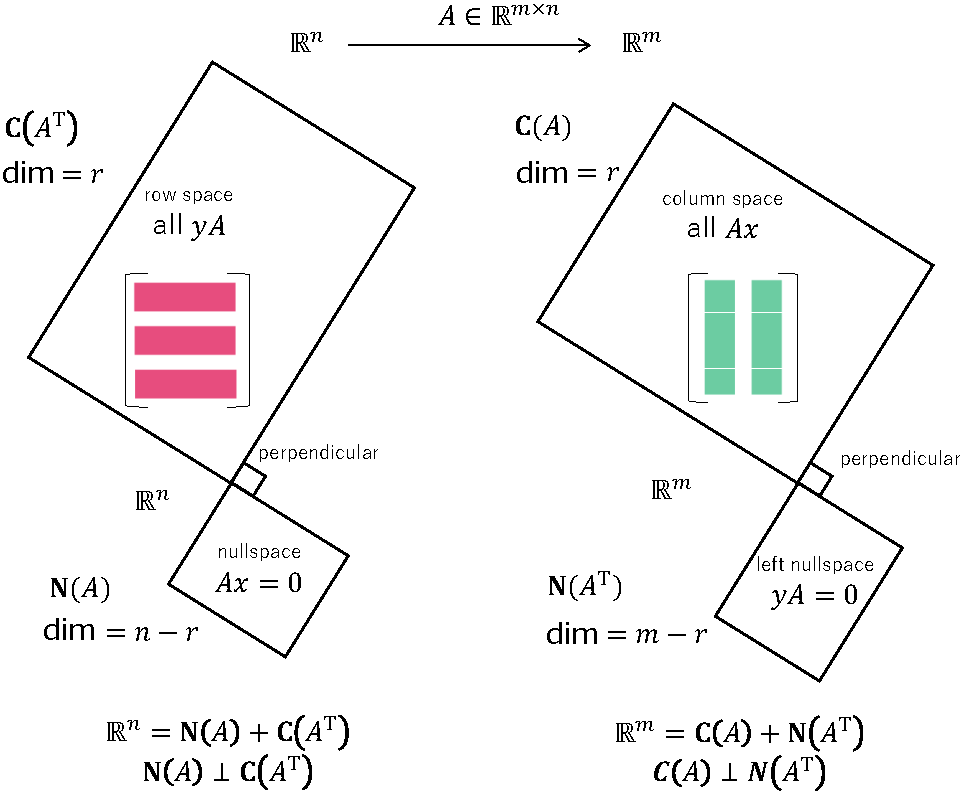
\includegraphics[width=13cm,height=10cm]{"figure/Question/四个子空间.png"}
	\caption{四个子空间}
\end{figure} 
\begin{solution}

	(1). 我们可以知道矩阵$A$的零空间为$N(A)=R^{n}$,我们可以得到$A$的行空间$R(A)=0$,$A=0$
	
	(2). 当$A$为反对称矩阵时,我们可以得到$\xi^{T}A\xi=0$
	
	(3). 我们不妨取$B=E$,可以得到$A=0$,矩阵$A$只能为零矩阵,在$A=0$时,任意的$n$阶矩阵$B$满足$AB=0$
	
	(4). 同$(3)$,取$B=E$,可以得到$A=0$,矩阵$A$只能为零矩阵,在$A=0$时,任意的$n$阶矩阵$B$满足$B^{T}AB=0$
\end{solution}
\myspace{1}

\hl{\textbf{\textit{August 6}}}

1.设函数$f(x)$在$(\dfrac{1}{2},+\infty)$上可导,且$\lim\limits_{h\rightarrow 0}\dfrac{f[(x+h)^2]-f(x^2+h)}{h}=1$,$f(1)=1$,求$f(x)$
\myspace{1}
\begin{solution}

	原极限等价于:  
	\begin{eqnarray*}
		I&=&\lim\limits_{h\rightarrow 0}\dfrac{f[(x+h)^2]-f(x^2+h)}{h}\\
		&=&\lim\limits_{h\rightarrow 0}\dfrac{f[(x+h)^2]-f(x^2)+f(x^2)-f(x^2+h)}{h}\\
		&=&\lim\limits_{h\rightarrow 0}\dfrac{f[(x+h)^2]-f(x^2)}{h}+\lim\limits_{h\rightarrow 0}\dfrac{f(x^2)-f(x^2+h)}{h}\\
		&=&[f(x^2)]'-f'(x^2)\\
		&=&(2x-1)f'(x^2)\\
		&=&1
	\end{eqnarray*}

	我们得到:  
	$$f'(x^2)=\dfrac{1}{2x-1}\Rightarrow 2xf'(x^2)=\dfrac{2x}{2x-1}\Rightarrow f(x^2)=x+\dfrac{1}{2}\ln(2x-1)+C$$
	
	我们由$f(1)=1\Rightarrow C=0\Rightarrow f(x^2)=x+\dfrac{1}{2}\ln(2x-1)$
	
	我们得到$f(x)=\sqrt{x}+\dfrac{1}{2}\ln(2\sqrt{x}-1)$
\end{solution}
\myspace{1}

2. $f(x)$在$[0,1]$上导函数连续,$f(0)=f(1)=0$,证明:  $\int_{0}^{1}f^{2}(x)dx\leq \dfrac{1}{8}\int_{0}^{1}[f'(x)]^2dx$
\myspace{1}
\begin{theorem}[积分形式柯西不等式]
	$$\left[ \int_{a}^{b}f(x)g(x)dx\right] ^2\leq \int_{a}^{b}f^2(x)dx\int_{a}^{b}g^{2}(x)dx$$
	
	我们知道$\forall t\in\mathbb{R}$,我们有:  
	$$\left[ tf(x)-g(x)\right]^2\geq 0\Rightarrow t^2f^{2}(x)-2tf(x)g(x)+g^{2}(x)\geq 0$$
	
	我们对上式子两边在区间$[a,b]$上积分,可以得到:  
	$$t^2\int_{a}^{b}f^{2}(x)dx-2t\int_{a}^{b}f(x)g(x)dx+\int_{a}^{b}g^{2}(x)dx\geq 0$$
	
	我们可以得到一个关于$t$的一元二次方程方程:  
	$$At^2+Bt+C\geq 0,\text{其中}\left\lbrace
	\begin{array}{l}
		A=\int_{a}^{b}f^{2}(x)dx\\
		B=-2\int_{a}^{b}f(x)g(x)dx\\
		C=\int_{a}^{b}g^{2}(x)dx
	\end{array}
	\right. \Rightarrow B^2-4AC\leq 0$$
	
	我们得到:  $$4\left[ \int_{a}^{b}f(x)g(x)dx\right]^2-4\int_{a}^{b}f^{2}(x)dx\int_{a}^{b}g^{2}(x)dx\leq 0 
	$$
	$$\left[ \int_{a}^{b}f(x)g(x)dx\right] ^2\leq \int_{a}^{b}f^2(x)dx\int_{a}^{b}g^{2}(x)dx$$
\end{theorem}
\begin{solution}

	我们知道:  $\left\lbrace
	\begin{array}{l}
		f(x)=\int_{0}^{x}f'(t)dt\\
		f(x)=\int_{1}^{x}f'(t)dt
	\end{array}
	\right. $
	我们有:  $$\int_{0}^{1}f^{2}(x)dx=\left\lbrace
	\begin{array}{l}
		\int_{0}^{1}\left[\int_{0}^{x}f'(t)dt \right]^2dx\leq \int_{0}^{1}[\int_{0}^{x}1^2dt\int_{0}^{x}|f'(t)|^2dt]dx\\
		\int_{0}^{1}\left[\int_{1}^{x}f'(t)dt \right]^2dx\leq \int_{0}^{1}[\int_{1}^{x}1^2dt\int_{0}^{x}|f'(t)|^2dt]dx
	\end{array}
	\right.$$
	
	我们可以得到:  
	\begin{eqnarray*}
		\int_{0}^{1}f^{2}(x)dx&=&\int_{0}^{\frac{1}{2}}f^{2}(x)dx+\int_{\frac{1}{2}}^{1}f^{2}(x)dx\\
		&=&\int_{0}^{\frac{1}{2}}\left[\int_{0}^{x}f'(t)dt \right]^2dx+\int_{\frac{1}{2}}^{1}\left[\int_{x}^{1}f'(t)dt \right]^2dx\\
		&\leq&\int_{0}^{\frac{1}{2}}[\int_{0}^{x}1^2dt\int_{0}^{x}|f'(t)|^2dt]dx+\int_{\frac{1}{2}}^{1}[\int_{x}^{1}1^2dt\int_{x}^{1}|f'(t)|^2dt]dx\\
		&\leq&\int_{0}^{\frac{1}{2}}[x\int_{0}^{x}|f'(t)|^2dt]dx+\int_{\frac{1}{2}}^{1}[(1-x)\int_{x}^{1}|f'(t)|^2dt]dx\\
		&=&\int_{0}^{\frac{1}{2}}|f'(t)|^2dt\int_{t}^{\frac{1}{2}}xdx+\int_{\frac{1}{2}}^{1}|f'(t)|^2dt\int_{\frac{1}{2}}^{t}(1-x)dx\\
		&=&(\dfrac{1}{8}-\dfrac{t^2}{2})\int_{0}^{\frac{1}{2}}|f'(t)|^2dt+(t-\dfrac{t^2}{2}-\dfrac{3}{8})\int_{\frac{1}{2}}^{1}|f'(t)|^2dt\\
		&=&\dfrac{1}{8}\int_{0}^{\frac{1}{2}}|f'(t)|^2dt+\dfrac{1}{8}\int_{\frac{1}{2}}^{1}|f'(t)|^2dt\\
		&=&\dfrac{1}{8}\int_{0}^{1}[f'(x)]^2dx
	\end{eqnarray*}
\end{solution}
\myspace{1}

3. 求$\lim\limits_{n\rightarrow+\infty}\left[\sqrt{n}(\sqrt{n+1}-\sqrt{n})+\dfrac{1}{2} \right]^{\dfrac{\sqrt{n+1}+\sqrt{n}}{\sqrt{n+1}-\sqrt{n}}} $
\myspace{1}
\begin{solution}

	原极限等价于:  
	\begin{eqnarray*}
		I&=&e^{\lim\limits_{n\rightarrow+\infty}\dfrac{\ln\left( 1+\dfrac{\sqrt{n}-\sqrt{n+1}}{2(\sqrt{n+1}+\sqrt{n})}\right)}{(\sqrt{n+1}-\sqrt{n})^2}}\\
		&=&e^{\lim\limits_{n\rightarrow+\infty}\dfrac{\dfrac{\sqrt{n}-\sqrt{n+1}}{2(\sqrt{n+1}+\sqrt{n})}}{(\sqrt{n+1}-\sqrt{n})^2}}\\
		&=&e^{\lim\limits_{n\rightarrow+\infty}-\dfrac{1}{2}}\\
		&=&e^{-\frac{1}{2}}
	\end{eqnarray*}
\end{solution}
\myspace{1}

\hl{\textbf{\textit{August 7}}}

1.设可导函数$y=y(x)$由方程$\sin x-\int_{x}^{y}\varphi(u)du=0$所确定,其中可导函数$\varphi(u)>0$,且$\varphi(0)=\varphi'(0)=1$,求$y''(0)$
\myspace{1}
\begin{solution}

	我们可以得到:  当$x=0$时,$\int_{0}^{y}\varphi(u)du=0$,且$\varphi(u)>0$,我们得到$y=0$.
	
	我们对方程$\sin x-\int_{x}^{y}\varphi(u)du=0$两边对$x$求导得到:  
	$$\left\lbrace
	\begin{array}{l}
		\cos x-[\varphi(y)y'-\varphi(x)]=0\\
		-\sin x-[\varphi'(y)y'^2+\varphi(y)y''-\varphi'(x)]=0
	\end{array}
	\right. \Rightarrow \left\lbrace
	\begin{array}{l}
		1-y'(0)\varphi(0)+\varphi(x)=0\\
		-\varphi'(0)y'(0)^2-y''(0)\varphi(0)+\varphi'(0)=0
	\end{array}
	\right. \Rightarrow \left\lbrace
	\begin{array}{l}
		y'(0)=2\\
		y''(0)=-3
	\end{array}
	\right. $$
\end{solution}
\myspace{1}

2.设$a_{n}=\int_{0}^{1}\dfrac{x^n}{1+x}dx$

(1).证明:  $\dfrac{1}{2(n+1)}\leq a_{n}\leq \dfrac{1}{2n},\ n=1,2,\cdots$

(2). 证明:  级数$\sum\limits_{n=1}^{+\infty}(-1)^{n-1}(\dfrac{1}{2n}-\int_{0}^{1}\dfrac{x^n}{1+x}dx)$绝对收敛.
\myspace{1}
\begin{solution}

	(1). 我们有:  $$\left\lbrace
	\begin{array}{l}
		\dfrac{x^n}{1+x}\geq \dfrac{x^n}{2},\ x\in(0,1)\\
		\dfrac{x^n}{1+x}=\dfrac{x}{1+x}x^{n-1}\leq\dfrac{x^{n-1}}{2},\ x\in(0,1)
	\end{array}
	\right. \Rightarrow \int_{0}^{1}\dfrac{x^n}{2}dx\leq \int_{0}^{1}\dfrac{x^n}{1+x}dx\leq \int_{0}^{1}\dfrac{x^{n-1}}{2}dx$$
	
	我们有:  $$\left\lbrace
	\begin{array}{l}
		\int_{0}^{1}\dfrac{x^n}{2}dx=\dfrac{x^{n+1}}{2(n+1)}|_{0}^{1}=\dfrac{1}{2(n+1)}\\
		\int_{0}^{1}\dfrac{x^{n-1}}{2}dx=\dfrac{x^{n}}{2n}|_{0}^{1}=\dfrac{1}{2n}
	\end{array}
	\right. $$
	
	我们证明了:  $\dfrac{1}{2(n+1)}\leq a_{n}\leq \dfrac{1}{2n},\ n=1,2,\cdots$
	
	(2). 我们不妨设$b_{n}=\dfrac{1}{2n}-a_{n}=\dfrac{1}{2n}-\int_{0}^{1}\dfrac{x^n}{1+x}dx$.
	
	我们由$(1)$可得:  $|b_{n}|\leq \dfrac{1}{2n}-\dfrac{1}{2(n+2)}=\dfrac{1}{2n^2+4n}<\dfrac{1}{2n^2}$
	
	我们知道级数$\sum\limits_{n=1}^{+\infty}\dfrac{1}{2n^2}$收敛,由比较判别法我们可知级数$\sum\limits_{n=1}^{+\infty}b_{n}$收敛,原级数绝对收敛.
\end{solution}
\myspace{1}

\section{Week \Rmnum{2}}
\hl{\textbf{\textit{August 8}}}

1.设$x=x(y)$是函数$y=\ln x+e^x$的反函数,求$\dfrac{d^2x}{dy^2}$.
\myspace{1}
\begin{solution}

	我们有:  $\left\lbrace
	\begin{array}{l}
		y=f(x)\\
		x=g(y)
	\end{array}
	\right. \Rightarrow \left\lbrace
	\begin{array}{l}
		y'(x)=f'(x)\\
		1=f'(x)g'(y)
	\end{array}
	\right. \Rightarrow g'(y)=\dfrac{1}{f(x)}$
	
	我们有:  $f(x)=\ln x+e^x\Rightarrow f'(x)=e^x+\dfrac{1}{x}$
	
	我们得到:  $g'(y)=\dfrac{dx}{dy}=\dfrac{1}{f(x)}=\dfrac{x}{1+xe^x}$
	
	我们有:  
	$$\dfrac{d^2x}{dy^2}=\dfrac{\dfrac{dx}{dy}}{dx}\dfrac{dx}{dy}=\dfrac{x-x^3e^x}{(1+xe^x)^3}$$
\end{solution}
\myspace{1}

2.设$a_{0}=1,a_{1}=0$,$a_{n+1}=\dfrac{1}{n+1}(na_{n}+a_{n-1})\ (n=1,2,3\cdots)$,$S(x)$为幂级数$\sum\limits_{n=0}^{+\infty}a_{n}x^{n}$的和函数.

(1).证明:  幂级数$\sum\limits_{n=0}^{+\infty}a_{n}x^n$的收敛半径不小于$1$.

(2).证明:  $(1-x)S'(x)-xS(x)=0,\ x\in(-1,1)$,并求出$S(x)$的表达式.
\myspace{1}
\begin{solution}

	(1). 我们由$a_{n+1}=\dfrac{1}{n+1}(na_{n}+a_{n-1})$得到:  
	$$a_{n+1}-a_{n}=-\dfrac{1}{n+1}(a_{n}-a_{n-1})$$
	
	我们不妨设$b_{n}=a_{n}-a_{n-1}\Rightarrow b_{n+1}=-\dfrac{1}{n+1}b_{n},\ b_{1}=a_{1}-a_{0}=-1$
	
	我们有:  $$\left\lbrace
	\begin{array}{l}
		b_{n}=-\dfrac{1}{n}b_{n-1}\\
		b_{n-1}=-\dfrac{1}{n-1}b_{n-2}\\
		\cdots\\
		b_{2}=-\dfrac{1}{2}b_{1}\\
		b_{1}=-1
	\end{array}
	\right. \Rightarrow b_{n}=\dfrac{(-1)^{n}}{n!}$$
	
	我们由累加法可以得到:  $a_{n}=\left\lbrace
	\begin{array}{l}
		a_{0}+\sum\limits_{k=1}^{n}b_{k}=\sum\limits_{k=0}^{n}\dfrac{(-1)^k}{k!},\ n\geq 1\\
		1,\ n=0
	\end{array}
	\right. \Rightarrow a_{n}=\sum\limits_{k=0}^{n}\dfrac{(-1)^k}{k!}$
	
	我们利用根值审敛法:  
	$$\rho=\lim\limits_{n\rightarrow+\infty}\sqrt[n]{a_{n}}=e^{\lim\limits_{n\rightarrow +\infty}\dfrac{\ln(\sum\limits_{k=0}^{n}\dfrac{(-1)^k}{k!})}{n}}=1$$
		
	我们得到级数的收敛半径:  $r=\dfrac{1}{\rho}=1$,幂级数$\sum\limits_{n=0}^{+\infty}a_{n}x^n$的收敛半径不小于$1$.

	(2). 我们有:  $S(x)=\sum\limits_{n=0}^{+\infty}a_{n}x^{n}$,我们得到:  
	$$\left\lbrace
	\begin{array}{l}
		S'(x)=\sum\limits_{n=1}^{+\infty}na_{n}x^{n-1}=\sum\limits_{n=0}^{+\infty}(n+1)a_{n+1}x^{n}\\
		S(x)=\sum\limits_{n=0}^{+\infty}a_{n}x^{n}
	\end{array}
	\right.$$
	
	$$a_{n+1}=\dfrac{1}{n+1}(na_{n}+a_{n-1})\Rightarrow (n+1)a_{n+1}=na_{n}+a_{n-1}\Rightarrow (n+2)a_{n+2}=(n+1)a_{n+1}=a_{n}$$
	
	我们得到:  
	\begin{eqnarray*}
		(1-x)S'(x)-xS(x)&=&(1-x)\sum\limits_{n=0}^{+\infty}(n+1)a_{n+1}x^{n}-x\sum\limits_{n=0}^{+\infty}a_{n}x^{n}\\
		&=&\sum\limits_{n=0}^{+\infty}(n+1)a_{n+1}x^{n}-\sum\limits_{n=0}^{+\infty}[(n+1)a_{n+1}+a_{n}]x^{n+1}\\
		&=&a_{1}+\sum\limits_{n=1}^{+\infty}(n+1)a_{n+1}x^{n}-\sum\limits_{n=0}^{+\infty}[(n+1)a_{n+1}+a_{n}]x^{n+1}\\
		&=&\sum\limits_{n=0}^{+\infty}(n+2)a_{n+2}x^{n+1}-\sum\limits_{n=0}^{+\infty}[(n+1)a_{n+1}+a_{n}]x^{n+1}\\
		&=&\sum\limits_{n=0}^{+\infty}[(n+2)a_{n+2}-(n+1)a_{n+1}-a_{n}]x^{n+1}\\
		&=&0
	\end{eqnarray*}
	
	我们得到:  
	$$(1-x)S'(x)-xS(x)=0\Rightarrow \dfrac{S'(x)}{S(x)}=\dfrac{x}{1-x}\Rightarrow S(x)=\dfrac{C_{1}}{e^x(1-x)}$$
	
	我们有$S(0)=1\Rightarrow C_{1}=1$,因此$S(x)=\dfrac{1}{e^x(1-x)},\ x\in(-1,1)$
	
\end{solution}
\myspace{1}

\hl{\textbf{\textit{August 9}}}

1.设$y=y(x)$由$e^y\sin t-y+1=0$和$x=\left\lbrace
\begin{array}{l}
	\dfrac{e^t-1}{t},\ t\neq 0\\
	1,\ t=0
\end{array}
\right. $所确定,求$\dfrac{d^2y}{dx^2}|_{t=0}$
\myspace{1}
\begin{solution}

	我们知道:  当$t=0$时,$\left\lbrace
	\begin{array}{l}
		x=1\\y=1
	\end{array}
	\right. $,我们由:  
	$$x(t)=\left\lbrace
	\begin{array}{l}
		\dfrac{e^t-1}{t},\ t\neq 0\\
		1,\ t=0
	\end{array}
	\right. \Rightarrow x(t)=1+\dfrac{t}{2}+\dfrac{t^2}{6}+\dfrac{t^3}{24}+\cdots\Rightarrow \left\lbrace
	\begin{array}{l}
		x'(0)=\dfrac{1}{2}\\
		x''(0)=\dfrac{1}{3}
	\end{array}
	\right. $$
	
	我们由:  $e^y\sin t-y+1=0\Rightarrow e^{y(t)}\sin t-y(t)+1=0$得到:  
	$$\left\lbrace
	\begin{array}{l}
		e^{y(t)}\cos t+y'(t)e^{y(t)}\sin t-y'(t)=0\\
		y'(t)e^{y(t)}\cos t-e^{y(t)}\sin t+\left\lbrace [y'(t)]^2e^{y(t)}+y''(t)e^{y(t)}\right\rbrace \sin x+\cos x\left[y'(t)e^{y(t)} \right]-y''(t)=0
	\end{array}
	\right.$$
	$$\left\lbrace
	\begin{array}{l}
		y'(0)=e\\
		y''(0)=2e^2
	\end{array}
	\right. $$
	
	我们由参数方程二阶导数公式:  
	$$\dfrac{d^2y}{dx^2}|_{t=0}=\dfrac{y''(t)x'(t)-x''(t)y'(t)}{[x'(t)]^3}|_{t=0}=8e^2-\dfrac{8e}{3}$$
	
\end{solution}
\myspace{1}

2. 下列命题正确的是:  
\begin{itemize}
	\item \hl{A}. 设$A$为$3$阶矩阵,若$A$的特征值$\lambda_{1}\lambda_{2}\neq 0,\lambda_{3}=0$,则$r(A)=2$
	\item \hl{B}. 设$A$为$3$阶非零矩阵,若$A^2=0$,则$r(A)=1$
	\item C. 设$A,B$为$3$阶矩阵,若$A$与$B$等价,则$|A|=|B|$
	\item D. 设$A,B$为$3$阶实对称矩阵,若$A$与$B$合同,则$|A|=|B|$
\end{itemize}
\myspace{1}
\begin{solution}

	(A). 我们可以得到矩阵$A\sim diag\{\lambda_{1},\lambda_{2},\lambda_{3}\}$,对角矩阵的秩和矩阵$A$的秩相同,$r(A)=2$
	
	(B). $A^2=0\Rightarrow 2r(A)\leq 3\Rightarrow r(A)=1$
	
	(C). $A$与$B$等价$\Rightarrow r(A)=r(B)$
	
	(D). $A$与$B$合同$\Rightarrow A=P^{T}BP$
\end{solution}
\myspace{1}

3.已知$f(x)=\left\lbrace
\begin{array}{l}
	\lim\limits_{n\rightarrow +\infty}\left( 1+\dfrac{2nx+x^2}{2n^2}\right)^{-n},\ x\neq 0\\
	\lim\limits_{n\rightarrow +\infty}2\left[ \dfrac{n}{(n+1)^2}+\dfrac{n}{(n+2)^2}+\cdots+\dfrac{n}{(n+n)^2}\right],\ x=0  
\end{array}
\right. $,求$\int f(x)dx$
\myspace{1}
\begin{solution}

	当$x\neq 0$时:  
	\begin{eqnarray*}
		f(x)&=&\lim\limits_{n\rightarrow +\infty}\left( 1+\dfrac{2nx+x^2}{2n^2}\right)^{-n}\\
		&=&e^{\lim\limits_{n\rightarrow +\infty}(-n)\dfrac{2nx+x^2}{2n^2}}\\
		&=&e^{-x}
	\end{eqnarray*}

	当$x=0$时:  
	\begin{eqnarray*}
		f(x)&=&\lim\limits_{n\rightarrow +\infty}2\left[ \dfrac{n}{(n+1)^2}+\dfrac{n}{(n+2)^2}+\cdots+\dfrac{n}{(n+n)^2}\right]\\
		&=&2\lim\limits_{n\rightarrow +\infty}\dfrac{1}{n}\left[ \dfrac{1}{(1+\dfrac{1}{n})^2}+\dfrac{1}{(1+\dfrac{2}{n})^2}+\cdots+\dfrac{1}{(1+\dfrac{n}{n})^2}\right]\\
		&=&2\int_{0}^{1}\dfrac{1}{(1+x)^2}dx\\
		&=&2(1-\dfrac{1}{2})\\
		&=&1
	\end{eqnarray*}

	我们得到:  $f(x)=e^{-x}\Rightarrow \int f(x)dx=-e^{-x}+C$
\end{solution}
\myspace{1}

\hl{\textbf{\textit{August 10}}}

1. 已知函数$f(x)=x^2\ln(1-x)$,当$n\geq 3$时,求$f^{(n)}(0)$
\myspace{1}
\begin{solution}

	我们利用$\ln(1-x)$的泰勒展开式:  
	$$\ln(1-x)=-x-\dfrac{x^2}{2}-\dfrac{x^3}{3}-\cdots-\dfrac{x^n}{n}-\cdots$$
	
	我们可以得到:  
	$$f(x)=-x^3-\dfrac{x^4}{2}-\dfrac{x^5}{3}-\cdots-\dfrac{x^n+2}{n}-\cdots$$
	
	我们有:  
	$$\left\lbrace
	\begin{array}{l}
		f'(0)=0\\
		f''(0)=0\\
		f^{(3)}(0)=-6\\
		f^{(4)}(0)=-\dfrac{4!}{2}\\
		\cdots\cdots
	\end{array}
	\right. \Rightarrow f^{(n)}(0)=-\dfrac{n!}{n-2},\ n\geq 3$$
\end{solution}
\myspace{1}

2. 设$f(x)$在$[0,1]$上可导,$f(0)=f(1)=-2$,证明:  $\exists \xi\in(0,1),\ s.t. f'(\xi)-f(\xi)=\xi$
\myspace{1}
\begin{solution}

	我们构造辅助函数:  $F(x)=e^{-x}\left[ f(x)+x+1\right]$,我们有:  
	$$F(0)=-1,\ F(1)=0,\ F'(x)=e^{-x}\left[ f'(x)-f(x)-x\right]$$
	
	我们由积分中值定理可以得到:  
	$$\exists \eta\in(0,1),\ s.t. \int_{0}^{1}f(x)dx=f(\eta)\Rightarrow \exists \eta\in(0,1),\ s.t. f(\eta)=0$$
	
	我们有:  
	$$F(\eta)=e^{-\eta}\left[ f(\eta)+\eta+1\right]=e^{-\eta}(\eta+1)>0$$
	
	我们根据零点定理,可知:  $\exists \delta\in(0,\eta),\ s.t. F(\delta)=0$.
	
	我们对$F(x)$在区间$[\delta,1]$上使用罗尔定理可以得到:  
	$$\exists\xi\in(\delta,1),\ s.t. F'(\xi)=e^{-\xi}\left[ f'(\xi)-f(\xi)-\xi\right]=0\Rightarrow f'(\xi)-f(\xi)=\xi$$
	
	综上所述,我们得到:  $\exists \xi\in(0,1),\ s.t. f'(\xi)-f(\xi)=\xi$
\end{solution}
\myspace{1}
\hl{\textbf{\textit{August 11}}}

1. 设数列$\{u_{n}\}$满足$u_{1}=1,\ u_{n+1}=\dfrac{u_{n}+3}{u_{n}+1},\ (n=1,2,\cdots)$,试证明数列$\{u_{n}\}$收敛,并求其极限.
\myspace{1}
\begin{solution}

	我们有:
	$$u_{1}=1,\ u_{2}=2,\ u_{3}=\dfrac{5}{3},\ u_{4}=\dfrac{7}{4},\cdots\ (u_{n}>0)$$
	
	我们发现数列$\{u_{n}\}$不是单调数列,我们从奇数项和偶数项入手:
	$$\left\lbrace
	\begin{array}{l}
		u_{2k+2}=\dfrac{u_{2k+1}+3}{u_{2k+1}+1}=\dfrac{\frac{u_{2k}+3}{u_{2k}+1}+3}{\frac{u_{2k}+3}{u_{2k}+1}+1}=2-\dfrac{1}{u_{2k}+2}\\
		u_{2k+1}=\dfrac{u_{2k}+3}{u_{2k}+1}=\dfrac{\frac{u_{2k-1}+3}{u_{2k-1}+1}+3}{\frac{u_{2k-1}+3}{u_{2k-1}+1}+1}=2-\dfrac{1}{u_{2k-1}+2}
	\end{array}
	\right. \Rightarrow f(x)=2-\dfrac{1}{x+2}\text{单调递增}$$
	
	我们首先证明数列$\{u_{2k-1}\}$极限存在:  
	
	(1). 当$n=1$时,$u_{1}<u_{3}$.
	
	(2). 当$n=k$时,假设$u_{2k-1}<u_{2k+1}$
	
	(3). 当$n=k+1$时,$u_{2k-1}<u_{2k+1}\Rightarrow f(u_{2k-1})<f(u_{2k+1})\Rightarrow u_{2k+1}<u_{2k+3}$
	
	数列$\{u_{2k-1}\},(k=1,2,\cdots)$单调递增,且$u_{2k-1}<2$
	
	我们继续证明数列$\{u_{2k}\}$极限存在:  
	
	(1). 当$n=1$时,$u_{2}>u_{4}$.
	
	(2). 当$n=k$时,假设$u_{2k}>u_{2k+2}$
	
	(3). 当$n=k+1$时,$u_{2k}>u_{2k+2}\Rightarrow f(u_{2k})>f(u_{2k+2})\Rightarrow u_{2k+2}<u_{2k+4}$
	
	数列$\{u_{2k}\},(k=1,2,\cdots)$单调递减少,且$u_{2k}>\dfrac{3}{2}$
	
	我们不妨假设:  $$\left\lbrace
	\begin{array}{l}
		\lim\limits_{k\rightarrow +\infty}u_{2k-1}=A\\
		\lim\limits_{k\rightarrow +\infty}u_{2k}=B\\
	\end{array}
	\right. \Rightarrow \left\lbrace
	\begin{array}{l}
		A=\dfrac{B+3}{B+1}\\
		B=\dfrac{A+3}{A+1}
	\end{array}
	\right. \Rightarrow A=B=\sqrt{3}$$
	
	我们可以得到:  
	
	(1). $\forall \varepsilon>0$,$\exists N_{1}>0$,当$n=2k-1>N_{1}$时,我们有:$|u_{2k-1}-\sqrt{3}|<\varepsilon$.
	
	(2). $\forall \varepsilon>0$,$\exists N_{2}>0$,当$n=2k>N_{2}$时,我们有:$|u_{2k}-\sqrt{3}|<\varepsilon$.
	
	(3). 取$N=\text{max}\{N_{1},N_{2}\}$,$\forall \varepsilon>0$,$\exists N>0$,当$n>N$时,我们有:$|u_{n}-\sqrt{3}|<\varepsilon$.
	
	综上所述,我们证明数列$\{u_{n}\}$收敛,极限为$\sqrt{3}$.
\end{solution}
\myspace{1}

2. $f(x)=\int_{1}^{x}\dfrac{\arctan t}{(1+t^2)^{\frac{3}{2}}\ln(1+t^2)}dt$,求$\int_{0}^{1}\dfrac{x}{1+x^2}f(x)dx$
\myspace{1}
\begin{solution}

	原定积分等价于:  
	\begin{eqnarray*}
		I&=&\int_{0}^{1}\dfrac{f(x)}{2}d(\ln(1+x^2))\\
		&=&\dfrac{f(x)\ln(1+x^2)}{2}|_{x=0}^{x=1}-\int_{0}^{1}\dfrac{\ln(1+x^2)}{2}d(f(x))\\
		&=&-\int_{0}^{1}\dfrac{\arctan x}{2(1+x^2)^{\frac{3}{2}}}dx\\
		&=&-\dfrac{1}{2}\int_{0}^{\frac{\pi}{4}}\theta\cos\theta d\theta\\
		&=&-\dfrac{1}{2}\theta\sin\theta|_{\theta=0}^{\theta=\frac{\pi}{4}}-\dfrac{1}{2}\int_{0}^{\frac{\pi}{4}}\sin \theta d\theta\\
		&=&-\dfrac{\sqrt{2}\pi}{16}+\dfrac{2-\sqrt{2}}{4}
	\end{eqnarray*}
\end{solution}
\myspace{1}

3. 设$f(x)=\dfrac{1}{1+2x+4x^2}$,求$f^{(100)}(0)$
\myspace{1}
\begin{solution}

	$$f(x)=\dfrac{1-2x}{(1-2x)(4x^2+2x+1)}=\dfrac{1-2x}{1-(2x)^3}$$
	$$\dfrac{1}{1-(2x)^3}=1+(2x)^3+(2x)^6+(2x)^9+\cdots+(2x)^{3n}$$
	
	我们得到:$$f(x)=(1-2x)\sum\limits_{n=0}^{+\infty}(2x)^{3n}=\sum\limits_{n=0}^{+\infty}(2x)^{3n}-\sum\limits_{n=0}^{+\infty}(2x)^{3n+1}$$
	$$f(x)=f(0)+f'(0)x+\cdots+\dfrac{f^{(n)}(0)}{n!}x^n$$
	
	$\dfrac{f^{(100)}(0)}{100!}$是$f(x)$中$x^{100}$前面的系数,我们可以得到:  
	$$f^{(100)}(0)=-2^{100}\times100!$$
\end{solution}
\myspace{1}

4. 证明:  在区间$(0,2)$内存在三个不同的点$x_{1},x_{2},x_{3}$,使得$\dfrac{1-\ln(1+x_{1})}{(1+x_{1})^2}x_{3}=\dfrac{1-\ln(1+x_{2})}{(1+x_{2})^2}(2-x_{3})$
\myspace{1}
\begin{solution}

	我们构造辅助函数:  $f(x)=\dfrac{\ln(1+x)}{1+x}$,我们有:  
	$$\left\lbrace 
	\begin{array}{l}
		f'(x)=\dfrac{1-\ln(1+x)}{(1+x)^2}\\
		f(0)=0\\
		f(2)=\dfrac{\ln 3}{3}
	\end{array}
	\right. $$
	
	我们不妨假设$\exists x_{3}\in(0,2), f(x_{3})=A$,我们分别在区间$(0,x_{3})$和区间$(x_{3},2)$上使用拉格朗日中值定理可以得到:  
	$$\left\lbrace 
	\begin{array}{l}
		\exists x_{1}\in(0,x_{3}),\ s.t. \dfrac{f(x_{3})-f(0)}{x_{3}}=f'(x_{1})=\dfrac{1-\ln(1+x_{1})}{(1+x_{1})^2}\\
		\exists x_{2}\in(x_{3},2),\ s.t. \dfrac{f(2)-f(x_{3})}{2-x_{3}}=f'(x_{2})=\dfrac{1-\ln(1+x_{2})}{(1+x_{2})^2}
	\end{array}
	\right. $$
	
	我们令$f(x_{3})-f(0)=f(2)-f(x_{3})\Rightarrow A=f(2)-A\Rightarrow f(x_{3})=A=\dfrac{f(2)}{2}=\dfrac{\ln 3}{6}$时,我们可以得到:  $$\dfrac{1-\ln(1+x_{1})}{(1+x_{1})^2}x_{3}=\dfrac{1-\ln(1+x_{2})}{(1+x_{2})^2}(2-x_{3})$$
	
	综上所述,我们可以得到:  在区间$(0,2)$内存在三个不同的点$x_{1},x_{2},x_{3}$,使得$\dfrac{1-\ln(1+x_{1})}{(1+x_{1})^2}x_{3}=\dfrac{1-\ln(1+x_{2})}{(1+x_{2})^2}(2-x_{3})$
\end{solution}
\myspace{1}

\hl{\textbf{\textit{August 12}}}

1. 设$y=\dfrac{\arcsin x}{\sqrt{1-x^2}}$

(1). 证明:  $(1-x^2)y^{(n+1)}-(2n+1)xy^{(n)}-n^2y^{(n-1)}=0(n\geq 1)$;

(2). 求$y^{(n)}(0)$
\myspace{1}
\begin{solution}

	(1). 我们对$f(x)$求导可以得到:  
	$$f'(x)=\dfrac{1+\dfrac{x\arcsin x}{\sqrt{1-x^2}}}{1-x^2}\Rightarrow f'(x)=\dfrac{1+xf(x)}{1-x^2}\Rightarrow (1-x^2)f'(x)-xf(x)-1=0$$
	
	我们令$g(x)=(1-x^2)f'(x)-xf(x)-1$,我们利用莱布尼兹公式可以得到:  
	$$g^{(n)}(x)=\sum\limits_{k=0}^{n}C_{n}^{k}(1-x^2)^{(k)}f^{(n-k+1)}(x)-\sum\limits_{k=0}^{n}C_{n}^{k}(x)^{(k)}f^{(n-k)}=0$$
	
	当$k\geq 3$时,$(1-x^2)^{(k)}=0$;当$k\geq 2$时,$x^{(k)}=0$,我们有:  
	$$g^{(n)}(x)=(1-x^2)f^{(n+1)}(x)-2nxf^{(n)}(x)-n(n-1)f^{(n-1)}(x)-xf^{(n)}(x)-nf^{(n-1)}(x)=0$$
	
	我们得到:  
	$$(1-x^2)f^{(n+1)}(x)-(2n+1)xf^{(n)}(x)-n^2f^{(n-1)}(x)=0$$
	
	综上所述,我们得到:  $(1-x^2)y^{(n+1)}-(2n+1)xy^{(n)}-n^2y^{(n-1)}=0(n\geq 1)$
	
	(2). 我们将$x=0$代入上面式子可以得到:  
	$$\left\lbrace 
	\begin{array}{l}
		y^{(n)}=(n-1)^2y^{(n-2)}\\
		y(0)=0\\
		y^{(1)}(0)=1
	\end{array}
	\right. \Rightarrow y^{(n)}(0)=\left\lbrace 
	\begin{array}{l}
		0,\ n\text{为偶数},n=2k(k=0,1,\cdots)\\
		(2k!!)^2,\ n\text{为奇数},n=2k+1(k=0,1,\cdots)
	\end{array}
	\right. $$
\end{solution}
\myspace{1}

2. 已知极限$\lim\limits_{t\rightarrow x}\left(\dfrac{\sin t}{\sin x} \right)^{\dfrac{x}{\sin t-\sin x}}$,记此极限为$f(x)$,求函数$f(x)$的间断点,并指出其类型.
\myspace{1}
\begin{solution}

	$$f(x)=e^{\lim\limits_{t\rightarrow x}\frac{x}{\sin t-\sin x}\ln(1+\frac{\sin t-\sin x}{\sin x})}=e^{\frac{x}{\sin x}}$$
	
	我们发现$f(x)$的间断点为$x=k\pi,\ k\in\mathbb{Z}$.
	
	(1). 当$k=0$时,我们有:
	$$\left\lbrace 
	\begin{array}{l}
		\lim\limits_{x\rightarrow 0^{+}}f(x)=e\\
		\lim\limits_{x\rightarrow 0^{-}}f(x)=e
	\end{array}
	\right. \Rightarrow x=0\text{是}f(x)\text{可去间断点}$$
	
	(2). 当$k\neq 0$时,我们有:
	$$\left\lbrace 
	\begin{array}{l}
		\lim\limits_{x\rightarrow k\pi^{+}}f(x)=+\infty\text{或者}0\\
		\lim\limits_{x\rightarrow 0^{-}}f(x)=0\text{或者}+\infty
	\end{array}
	\right. \Rightarrow x=k\pi\text{是}f(x)\text{无穷间断点}$$
\end{solution}
\myspace{1}

3. 证明:  $\int_{0}^{\pi}xa^{\sin x}dx\int_{0}^{\frac{\pi}{2}}a^{-\cos x}dx\geq \dfrac{\pi^3}{4}$
\myspace{1}
\begin{solution}

	我们由区间再现公式可以得到:
	$$\left\lbrace 
	\begin{array}{l}
		I_{1}=\int_{0}^{\pi}(\pi-t)a^{\sin t}dt\\
		2I_{1}=\pi\int_{0}^{\pi}a^{\sin t}dt\\
		I_{1}=\pi\int_{0}^{\frac{\pi}{2}}a^{\cos t}dt
	\end{array}
	\right. $$
	
	我们可以得到原定积分等价于:(柯西不等式)
	\begin{eqnarray*}
		\text{左边}&=&\pi\int_{0}^{\frac{\pi}{2}}a^{\cos x}dx\int_{0}^{\frac{\pi}{2}}a^{-\cos x}dx\\
		&=&\pi\int_{0}^{\frac{\pi}{2}}f^{2}(x)dx\int_{0}^{\frac{\pi}{2}}g^{2}(x)dx\\
		&\geq &\pi \left[ \int_{0}^{\frac{\pi}{2}}f(x)g(x)dx\right]^2\\
		&=&\dfrac{\pi^3}{4} 
	\end{eqnarray*}
\end{solution}
\myspace{1}

\hl{\textbf{\textit{August 13}}}

1. 设函数$f(x)=\left\lbrace
\begin{array}{l}
	x|x|,\ x\leq 0,\\
	x\ln x,\ x>0,
\end{array}
\right. $,\ $x=0$处$f(x)$的可导性判断、$x=0$是否为$f(x)$的极值点
\myspace{1}
\begin{solution}

	当$x=0$时,我们有$f(0)=0$,且我们有:  
	$$\left\lbrace
	\begin{array}{l}
		\lim\limits_{x\rightarrow 0^{+}}f(x)=\lim\limits_{x\rightarrow 0^{+}}x\ln x=0\\
		\lim\limits_{x\rightarrow 0^{-}}f(x)=\lim\limits_{x\rightarrow 0^{-}}(-x^2)=0
	\end{array}
	\right. \Rightarrow \lim\limits_{x\rightarrow 0}f(x)=f(0)\Rightarrow f(x)\text{在}x=0\text{处连续}$$
	
	我们有:  
	$$\left\lbrace
	\begin{array}{l}
		\lim\limits_{x\rightarrow 0^{+}}\dfrac{f(x)-f(0)}{x}=\ln x=-\infty\\
		\lim\limits_{x\rightarrow 0^{-}}\dfrac{f(x)-f(0)}{x}=-x=0
	\end{array}
	\right. \Rightarrow f(x)\text{在}x=0\text{处不可导}$$
	
	取$\varepsilon\in(0,1)$,当$x\in(-\varepsilon,0)$时,$f(x)=-x^2<f(0)=0$;当$x\in(0,\varepsilon)$时,$f(x)=x\ln x<f(0)=0$,$x=0$是$f(x)$的极大值点.
\end{solution}
\myspace{1}

2. 已知$f(x)=\prod\limits_{n=1}^{100}\left(\tan\dfrac{\pi x^n}{4}-n\right)$,求$f'(1)$
\myspace{1}
我们令$g(x)=\prod\limits_{n=2}^{100}\left(\tan\dfrac{\pi x^n}{4}-n\right)$,我们得到:$$f(x)=(\tan\dfrac{\pi x}{4}-1)g(x)$$
$$f'(x)=\dfrac{\pi}{4\cos^2\frac{\pi x}{4}}g(x)+g'(x)(\tan\dfrac{\pi x}{4}-1)$$
$$f'(1)=\dfrac{\pi}{2}g(1)=\dfrac{\pi}{2}\times(1-2)\times(1-3)\cdots\times(1-100)=-\dfrac{\pi}{2}99!$$
\myspace{1}

\hl{\textbf{\textit{August 14}}}

1. 已知函数$f(x)=\left\lbrace
\begin{array}{l}
	\int_{0}^{x}\cos\dfrac{1}{t}dt,\ x\neq 0\\
	0,\ x=0
\end{array}
\right. $,求$f'(0)$
\myspace{1}
\begin{solution}

	我们有:$\lim\limits_{x\rightarrow 0}f(x)=f(0)=0$,我们根据导数的定义可以得到:  
	\begin{eqnarray*}
		f'(0)&=&\lim\limits_{x\rightarrow 0}\dfrac{\int_{0}^{x}\cos\dfrac{1}{t}dt}{x}\\
		&=&\lim\limits_{x\rightarrow 0}-\dfrac{\int_{0}^{x}t^2d\sin\dfrac{1}{t}}{x}\\
		&=&\lim\limits_{x\rightarrow 0}\left[ -t\sin\dfrac{1}{t}|_{t=0}^{t=x}\right]+\lim\limits_{x\rightarrow 0}\dfrac{\int_{0}^{x}2t\sin\dfrac{1}{t}dt}{x}\\
		&=&0+2\lim\limits_{x\rightarrow 0}x\sin\dfrac{1}{x}\\
		&=&0
	\end{eqnarray*}

	综上所述,我们得到:$f'(0)=0$
\end{solution}
\myspace{1}

2. $f(x)$可导,且满足$x=\int_{0}^{x}f(t)dt+\int_{0}^{x}tf(t-x)dt$,求$f(x)$以及$\int_{-\frac{\pi}{4}}^{\frac{3\pi}{4}}|f(x)|^6dx$
\myspace{1}
\begin{solution}

	我们令$u=t-x,t=u+x$,我们得到:
	$$x=\int_{0}^{x}f(t)dt+\int_{-x}^{0}(u+x)f(u)du\Rightarrow x=\int_{0}^{x}f(t)dt+\int_{-x}^{0}uf(u)du+x\int_{-x}^{0}f(u)du$$
	
	我们对方程左右两边对$x$求导,得到:
	$$1=f(x)-xf(-x)+\int_{-x}^{0}f(u)du+xf(-x)\Rightarrow f(x)+\int_{-x}^{0}f(u)du=1$$
	
	我们再求一次导数,得到:  
	$$f'(x)+f(-x)=0\Rightarrow f''(x)-f'(-x)=0\Rightarrow f''(x)=f(x)$$
	
	我们得到特征方程:$\lambda^2+1=0\Rightarrow \lambda_{1}=i,\lambda_{2}=-i$
	
	我们不妨设$f(x)=C_{1}\sin x+C_{2}\cos x$
	
	我们有:$\left\lbrace
	\begin{array}{l}
		f(0)=1\\
		f'(1)=-1
	\end{array}
	\right. \Rightarrow \left\lbrace
	\begin{array}{l}
		C_{1}=-1\\
		C_{2}=1
	\end{array}
	\right. \Rightarrow f(x)=\cos x-\sin x=\sqrt{2}\cos(x+\frac{\pi}{4})$
	
	我们得到:
	\begin{eqnarray*}
		\int_{-\frac{\pi}{4}}^{\frac{3\pi}{4}}|f(x)|^6dx&=&8\int_{-\frac{\pi}{4}}^{\frac{3\pi}{4}}\cos^6(x+\frac{\pi}{4})dx\\
		&=&8\int_{0}^{\pi}\cos^6 tdt\\
		&=&16\int_{0}^{\frac{\pi}{2}}\cos^6 tdt\\
		&=&16\times\dfrac{5}{6}\times\dfrac{3}{4}\times\dfrac{1}{2}\times\dfrac{\pi}{2}\\
		&=&\dfrac{5\pi}{2}
	\end{eqnarray*}
\end{solution}
\myspace{1}

3. 设函数$f(x)=\int_{-1}^{x}t\ln|t|dt$,\ $x=0$处$f(x)$的可导性判断、$x=0$是否为$f(x)$的极值点
\myspace{1}
\begin{solution}

	我们有$g(x)=x\ln|x|$在$x=0$处可去间断,且$\lim\limits_{x\rightarrow 0}g(x)=0$,我们得到$f(x)$在$x=0$处连续
	
	我们有:
	$$\left\lbrace
	\begin{array}{l}
		\lim\limits_{x\rightarrow 0^{+}}\dfrac{f(x)-f(0)}{x}=\dfrac{\int_{0}^{x}t\ln tdt}{x}=\lim\limits_{x\rightarrow 0^{+}}x\ln x=0\\
		\lim\limits_{x\rightarrow 0^{-}}\dfrac{f(x)-f(0)}{x}=\dfrac{\int_{x}^{0}t\ln(-t)dt}{x}=\lim\limits_{x\rightarrow 0^{+}}(-x)\ln(-x)=0
	\end{array}
	\right. \Rightarrow f'(0)=0$$
	
	当$x\in(-1,0)$时,$f(x)>f(0)$;当$x\in(0,1)$时,$f(x)>f(0)$,$f(x)$在$x=0$处取极小值.
\end{solution}
\myspace{1}

\section{Week \Rmnum{3}}
\hl{\textbf{\textit{August 15}}}

1. 函数$f(x)=(x+1)|x^2-1|$驻点和极值点个数
\myspace{1}
\begin{solution}

	我们得到:  $f(x)=\left\lbrace
	\begin{array}{l}
		x^3+x^2-x-1,\ |x|\geq 1\\
		x+1-x^2-x^3,\ |x|<1
	\end{array}
	\right. $,我们对$f(x)$求导得到:
	$$f'(x)=\left\lbrace
	\begin{array}{l}
		3x^2+2x-1,\ x\leq -1\\
		1-2x-3x^2,\ -1<x<1\\
		3x^2+2x-1,\ x>1
	\end{array}
	\right. \Rightarrow f(x)\text{在}x=-1\text{处可导};\text{在}x=1\text{处不可导}$$
	$$f'(x)=\left\lbrace
	\begin{array}{l}
		(3x-1)(x+1),\ x\leq -1\\
		(1-3x)(x+1),\ -1<x<1\\
		(3x-1)(x+1),\ x>1
	\end{array}
	\right.$$
	
	我们发现:  
	$$\left\lbrace
	\begin{array}{l}
		x\in(-\infty,-1),f'(x)>0\\
		x\in(-1,\dfrac{1}{3}),f'(x)>0\\
		x\in(\dfrac{1}{3},1),f'(x)<0\\
		x\in(1,+\infty),f'(x)>0
	\end{array}
	\right. $$
	
	在可导点处,$f(x)$有两个驻点$x=\dfrac{1}{3}$和$x=-1$;$f(x)$有一个极值点$x=\dfrac{1}{3}$.
	
	在不可导点$x=1$处,$x=1$不是驻点,$x=1$两侧导数值异号,$x=1$是极值点.
	
	综上所述,我们得到$f(x)$有$x=\dfrac{1}{3}$和$x=-1$两个驻点和$x=\dfrac{1}{3}$和$x=1$两个极值点.
	
\end{solution}
\myspace{1}

2. 已知函数$f(x)$在$x=0$的某个邻域内二阶可导,且$\lim\limits_{x\rightarrow 0 }\left[ \dfrac{\sin x}{x^3}+\dfrac{f(x)}{x^2}\right]=\dfrac{1}{3}$,求$f(0)$、$f'(0)$及$f''(0)$
\myspace{1}
\begin{solution}

	原极限等价于:  
	\begin{eqnarray*}
		I&=&\lim\limits_{x\rightarrow 0 } \dfrac{\sin x-x+xf(x)+x}{x^3}\\
		&=&\lim\limits_{x\rightarrow 0 } \dfrac{\sin x-x}{x^3}+\lim\limits_{x\rightarrow 0 } \dfrac{f(x)+1}{x^2}\\
		&=&-\dfrac{1}{6}+\lim\limits_{x\rightarrow 0 } \dfrac{f(x)+1}{x^2}\\
		&=&\dfrac{1}{3}
	\end{eqnarray*}

	我们得到:  $\lim\limits_{x\rightarrow 0 } \dfrac{f(x)+1}{x^2}=\dfrac{1}{2}$
	
	我们得到:  
	$$\left\lbrace
	\begin{array}{l}
		f(0)=-1\\
		\lim\limits_{x\rightarrow 0}\dfrac{f'(x)}{2x}=\dfrac{1}{2}\\
		\lim\limits_{x\rightarrow 0}\dfrac{f''(x)}{2}=\dfrac{1}{2}
	\end{array}
	\right. \Rightarrow \left\lbrace
	\begin{array}{l}
		f(0)=-1\\
		f'(0)=0\\
		f''(0)=1
	\end{array}
	\right. $$
\end{solution}
\myspace{1}

3. 设$f(x)$连续,且$x>1$时,我们有$f(x)\left[ \int_{0}^{x}f(t)dt+1\right]=\dfrac{xe^x}{2(1+x)^2}$,求$f(x)$
\myspace{1}
\begin{solution}

	我们不妨设$F(x)=\int_{0}^{x}f(t)dt\Rightarrow F'(x)=f(x)$
	
	我们构造辅助函数:$G(x)=\left[F(x)+1\right]^2\Rightarrow G'(x)=\dfrac{xe^x}{(1+x)^2}$
	
	我们可以得到:  $\left\lbrace
	\begin{array}{l}
		G(x)=\dfrac{e^x}{1+x}+C\\ G(0)=[F(0)+1]^2=1
	\end{array}
	\right. \Rightarrow C=0$
	
	我们得到:  $$\left\lbrace
	\begin{array}{l}
		F(x)+1=\sqrt{\dfrac{e^x}{1+x}}\\
		f(x)=F'(x)=\dfrac{xe^{\frac{x}{2}}}{2(1+x)^{\frac{3}{2}}}
	\end{array}
	\right. $$
	
	综上所述,我们得到:  $f(x)=\dfrac{xe^{\frac{x}{2}}}{2(1+x)^{\frac{3}{2}}}$
\end{solution}
\myspace{1}

\hl{\textbf{\textit{August 16}}}

1. 设$f(x)$有二阶连续导数,且$f'(0)=0$,$\lim\limits_{x\rightarrow 0}\dfrac{f''(x)+f(x)-f(-x)}{|x|}=1$,下列说法正确的是:
\begin{itemize}
	\item A. $f(0)$是$f(x)$极大值
	\item B. $f''(0)>0$,$f(0)$是$f(x)$极小值
	\item C. $(0,f(0))$是曲线$y=f(x)$的拐点
	\item \hl{D}. $f(0)$是$f(x)$的极值点,$(0,f(0))$不是曲线$y=f(x)$的拐点
\end{itemize}
\myspace{1}
\begin{solution}

	原极限等价于:  
	\begin{eqnarray*}
		I&=&\lim\limits_{x\rightarrow 0}\dfrac{f''(x)+f(x)-f(-x)}{|x|}\\
		&=&\lim\limits_{x\rightarrow 0}\dfrac{f''(x)+\left[f(0)+f'(0)x+o(x)\right] -\left[ f(0)-f'(0)x+o(x)\right]}{|x|}\\
		&=&\lim\limits_{x\rightarrow 0}\dfrac{f''(x)+2f'(0)x+o(x)}{|x|}\\
		&=&\lim\limits_{x\rightarrow 0}\dfrac{f''(x)}{|x|}\\
		&=&1
	\end{eqnarray*}

	我们得到:$f''(0)=0$,且$x\in(-\xi,\xi)$,$f''(x)>0$,我们知道$f'(x)$在$x\in(-\xi,\xi)$上单调递增,$x=0$是$f(x)$的极小值点,$(0,f(0))$不是函数$f(x)$的拐点.
\end{solution}
\myspace{1}

2. 计算极限$$\lim\limits_{t\rightarrow 0^{+}}\dfrac{1}{t^3}\int_{0}^{\frac{\pi}{4}}d\theta\int_{0}^{\frac{t}{\cos \theta}}\dfrac{\sin(r^2\sin\theta\cos\theta)}{\sin\theta}dr$$
\myspace{1}
\begin{solution}

	原极限等价于:  
	\begin{eqnarray*}
		I&=&\lim\limits_{t\rightarrow 0^{+}}\dfrac{1}{t^3}\int_{0}^{\frac{\pi}{4}}d\theta\int_{0}^{\frac{t}{\cos \theta}}\dfrac{\sin(r^2\sin\theta\cos\theta)}{r\sin\theta}rdr\\
		&=&\lim\limits_{t\rightarrow 0^{+}}\dfrac{\int_{0}^{t}dx\int_{0}^{x}\dfrac{\sin(xy)}{y}dy}{t^3}\\
		&=&\lim\limits_{t\rightarrow 0^{+}}\dfrac{\int_{0}^{t^2}\dfrac{\sin u}{u}du}{3t^2}\\
		&=&\lim\limits_{t\rightarrow 0^{+}}\dfrac{2t\sin(t^2)}{6t^3}\\
		&=&\dfrac{1}{3}
	\end{eqnarray*}
\end{solution}
\myspace{1}

3. 设$f(x)$连续,且$f(x)\neq 0,f(1)=\sqrt{2}$,若对任意$x,y\in(-\infty,+\infty)$,有$f(x+y)-f(x)=\int_{x}^{x+y}\dfrac{t}{f(t)}(t^2+1)dt$,求$f(x)$
\myspace{1}
\begin{solution}

	我们可以得到:
	\begin{eqnarray*}
		f'(x)&=&\lim\limits_{\Delta x\rightarrow 0}\dfrac{f(x+\Delta)-f(x)}{\Delta x}\\
		&=&\lim\limits_{\Delta x\rightarrow 0}\dfrac{\int_{x}^{x+\Delta x}\dfrac{t}{f(t)}(t^2+1)dt}{\Delta x}\\
		&=&\lim\limits_{\Delta x\rightarrow 0}\dfrac{(x+\Delta x)}{f(x+\Delta x)}\left[ (x+\Delta x)^2+1\right] \\
		&=&\dfrac{x(x^2+1)}{f(x)}
	\end{eqnarray*}

	我们得到:  $f'(x)f(x)=x^3+x\Rightarrow [f^2(x)]'=2x^3+2x$
	
	我们得到:  $f^{2}(x)=\dfrac{x^4}{2}+x^2+C,\ f(1)=\sqrt{2}\Rightarrow C=\dfrac{1}{2}$
	
	我们得到:  $f(x)=\sqrt{\dfrac{x^4}{2}+x^2+\dfrac{1}{2}}=\dfrac{x^2+1}{\sqrt{2}}$
\end{solution}
\myspace{1}

4. 设$f(x)$在$[0,+\infty)$连续,在$(0,+\infty)$恒正,$x>0$时,我们有$\left[ f(x)\right]^3\leq 3\int_{0}^{x}f^{2}(t)dt$,证明:$x\geq 0\text{时,均有}f(x)\leq x$
\myspace{1}
\begin{solution}

	我们构造辅助函数:  $F(x)=\int_{0}^{x}f^{2}(t)dt,\ F'(x)=f^{2}(x)$
	
	我们得到:  $$[F'(x)]^{\frac{3}{2}}\leq 3F(x)\Rightarrow F'(x)\leq 3^{\frac{2}{3}}[F(x)]^{\frac{2}{3}}\Rightarrow \dfrac{F'(x)}{[F(x)]^{\frac{2}{3}}}\leq 3^{\frac{2}{3}}$$
	
	我们构造:  $G(x)=F(x)^{\dfrac{1}{3}},\ G'(x)=\dfrac{F'(x)}{3[F(x)]^{\frac{2}{3}}}\leq 3^{-\frac{1}{3}}$
	
	我们得到:$G(x)\leq \int_{0}^{x}3^{-\frac{1}{3}}=3^{-\frac{1}{3}}x\Rightarrow F(x)^{\frac{1}{3}}\leq3^{-\frac{1}{3}}x$
	
	我们有:$$F'(x)\leq 3^{\frac{2}{3}}[F(x)]^{\frac{2}{3}}\Rightarrow f^{2}(x)\leq x^2\Rightarrow f(x)\leq x$$

	我们补充$\lim\limits_{x\rightarrow 0}f(x)=0$,综上所述,我们得到:  $x\geq 0\text{时,均有}f(x)\leq x$	
	
\end{solution}
\myspace{1}

\hl{\textbf{\textit{August 17}}}

1. 已知$f(x)=\dfrac{x|x|}{1+x}$,求$f(x)$的凹凸区间以及渐近线
\myspace{1}
\begin{solution}

	我们有:  
	$$f'(x)=\left\lbrace
	\begin{array}{l}
		\dfrac{x^2+2x}{(1+x)^2},\ x\geq 0\\
		-\dfrac{x^2+2x}{(1+x)^2},\ x<0,\text{且}x\neq -1
	\end{array}
	\right. \Rightarrow f''(x)=\left\lbrace
	\begin{array}{l}
		\dfrac{2}{(1+x)^3},\ x>0\\
		-\dfrac{2}{(1+x)^3},\ x<0,\text{且}x\neq -1
	\end{array}
	\right. $$
	
	$f'(0)=0$,我们利用导数定义得到:  
	$$\left\lbrace
	\begin{array}{l}
		\lim\limits_{x\rightarrow 0^{+}}\dfrac{f'(x)}{x}=2\\
		\lim\limits_{x\rightarrow 0^{-}}\dfrac{f'(x)}{x}=-2
	\end{array}
	\right. \Rightarrow f''(x)\text{在}x=0\text{跳跃间断}$$
	
	当$x\in(0,+\infty)$,$f''(x)>0$,我们可以得到:$(0,+\infty)$是$f(x)$的凹区间;
	
	当$x\in(-\infty,-1)$,$f''(x)>0$,我们可以得到:$(-\infty,-1)$是$f(x)$的凹区间;
	
	当$x\in(-1,0)$,$f''(x)<0$,我们可以得到:$(-1,0)$是$f(x)$的凸区间.
	
	铅锤渐近线:$x=-1$;无水平渐近线
	
	斜渐近线:  
	
	(1).
	$$\left\lbrace
	\begin{array}{l}
		a=\lim\limits_{x\rightarrow+\infty}\dfrac{f(x)}{x}\\
		b=\lim\limits_{x\rightarrow+\infty}(f(x)-ax)
	\end{array}
	\right. \Rightarrow\left\lbrace
	\begin{array}{l}
		a=1\\
		b=-1
	\end{array}
	\right. $$
	
	(2).
	$$\left\lbrace
	\begin{array}{l}
		a=\lim\limits_{x\rightarrow-\infty}\dfrac{f(x)}{x}\\
		b=\lim\limits_{x\rightarrow-\infty}(f(x)-ax)
	\end{array}
	\right. \Rightarrow\left\lbrace
	\begin{array}{l}
		a=-1\\
		b=1
	\end{array}
	\right. $$
	
	综上所述,$f(x)$有三条渐近线,铅锤渐近线$x=-1$;斜渐近线$y=x-1$和$y=-x+1$.
\end{solution}
\myspace{1}

2. 函数$f(x)$具有二阶连续的导数,曲线$y=f(x)$既关于$y$轴对称也关于直线$x=1$对称,求$\int_{-2}^{2}(x-2024)f''(x)dx$
\myspace{1}
\begin{solution}

	周期性、轴对称性、中心对称性
	
	我们可以得到$f(x)$是以$T=2$为周期的周期函数;且$f(x)$是偶函数,$f'(x)$是奇函数且为周期函数.
	
	原定积分等价于:  
	\begin{eqnarray*}
		I&=&\int_{-2}^{2}(x-2024)df'(x)\\
		&=&(x-2024)f'(x)|_{x=-2}^{x=2}-\int_{-2}^{2}f'(x)dx\\
		&=&0
	\end{eqnarray*}
\end{solution}
\myspace{1}

3. 设$(X,Y)$的概率密度为$f(x,y)=\left\lbrace
\begin{array}{l}
	x+y,\ 0\leq x\leq 1,\ 0\leq y\leq 1\\
	0,\ \text{其他}
\end{array}
\right. $

(1). 求$\text{max}\{X,Y\}$的分布函数和概率密度

(2). 求$\text{min}\{X,Y\}$的分布函数和概率密度
\myspace{1}
\begin{solution}
	
\end{solution}
\myspace{1}

\hl{\textbf{\textit{August 18}}}

1. 曲线$y=x(1+\arcsin \dfrac{2}{x})$的斜渐近线方程
\myspace{1}
\begin{solution}

	(1). $x\Rightarrow +\infty$
	
	$$\left\lbrace
	\begin{array}{l}
		a=\lim\limits_{x\rightarrow+\infty}\dfrac{f(x)}{x}=\lim\limits_{x\rightarrow+\infty}(1+\arctan\dfrac{2}{x})\\
		b=\lim\limits_{x\rightarrow+\infty}(f(x)-ax)=\lim\limits_{x\rightarrow+\infty}x\arctan\dfrac{2}{x}
	\end{array}
	\right. \Rightarrow \left\lbrace
	\begin{array}{l}
		a=1\\
		b=2
	\end{array}
	\right. $$
	
	(2). $x\Rightarrow -\infty$
	
	$$\left\lbrace
	\begin{array}{l}
		a=\lim\limits_{x\rightarrow-\infty}\dfrac{f(x)}{x}=\lim\limits_{x\rightarrow -\infty}(1+\arctan\dfrac{2}{x})\\
		b=\lim\limits_{x\rightarrow-\infty}(f(x)-ax)=\lim\limits_{x\rightarrow-\infty}x\arctan\dfrac{2}{x}
	\end{array}
	\right. \Rightarrow \left\lbrace
	\begin{array}{l}
		a=1\\
		b=2
	\end{array}
	\right. $$
	
	综上所述,$f(x)$的斜渐近线方程为:$y=x+2$
\end{solution}
\myspace{1}

2. $\int_{0}^{1}\dfrac{\arcsin\sqrt{x}}{x^2-x+1}dx$
\myspace{1}
\begin{solution}

	我们有:$\left\lbrace
	\begin{array}{l}
		\sin\theta=\sqrt{x}\\
		\cos\theta=\sqrt{1-x}
	\end{array}
	\right. \Rightarrow \left\lbrace
	\begin{array}{l}
		\arcsin\sqrt{x}=\theta\\
		\arcsin\sqrt{1-x}=\dfrac{\pi}{2}-\theta
	\end{array}
	\right. $
	我们利用区间再现公式得到:  
	\begin{eqnarray*}
		I&=&\int_{0}^{1}\dfrac{\arcsin\sqrt{1-x}}{x^2-x+1}dx\\
		2I&=&\int_{0}^{1}\dfrac{\pi}{2(x^2-x+1)}dx\\
		I&=&\dfrac{\pi}{4}\int_{0}^{1}\dfrac{\pi}{(x-\frac{1}{2})^2+\frac{3}{4}}dx\\
		&=&\dfrac{\pi}{4}\dfrac{2}{\sqrt{3}}\arctan\dfrac{2x-1}{\sqrt{3}}|_{x=0}^{x=1}\\
		&=&\dfrac{\sqrt{3}\pi^2}{18}
	\end{eqnarray*}
\end{solution}
\myspace{1}

3. $\int_{0}^{\frac{\pi}{4}}\ln(1+\tan x)dx$
\myspace{1}
\begin{solution}

	我们利用区间再现公式得到:
	\begin{eqnarray*}
		I&=&\int_{0}^{\frac{\pi}{4}}\ln(1+\dfrac{1-\tan x}{1+\tan x})dx\\
		&=&\int_{0}^{\frac{\pi}{4}}\ln(\dfrac{2}{1+\tan x})dx\\
		2I&=&\int_{0}^{\frac{\pi}{4}}\ln2dx\\
		I&=&\dfrac{\pi \ln2}{8}
	\end{eqnarray*}
\end{solution}
\myspace{1}

4. 设$f(x)=\arctan x$,求$f^{(n)}(0)$($n$为奇数)
\myspace{1}
\begin{solution}

	我们利用泰勒展开式:
	$$(\arctan x)'=\dfrac{1}{1+x^2}=1-x^2+x^4+\cdots+(-1)^{n-1}x^{2n-2}$$
	$$\left\lbrace
	\begin{array}{l}
		f(x)=\arctan x=x-\dfrac{x^3}{3}+\dfrac{x^5}{5}-\cdots+\dfrac{(-1)^{n-1}x^{2n-1}}{2n-1}\\
		f(x)=f(0)+f'(0)x+\dfrac{f''(0)}{2!}x^2+\cdots+\dfrac{f^{(n)}(0)}{n!}+\cdots
	\end{array}
	\right. $$
	
	我们可以得到:$\dfrac{f^{(n)}(0)}{n!}=\dfrac{(-1)^{\frac{n-1}{2}}}{n}\Rightarrow f^{(n)}(0)=(-1)^{\frac{n-1}{2}}(n-1)!$
		
	综上所述,我们得到:  $f^{(n)}(0)=(-1)^{\frac{n-1}{2}}(n-1)!,\ n\text{为奇数}$
\end{solution}
\myspace{1}

5. 设$f(x)=\left\lbrace
\begin{array}{l}
	ax+1,\ x<0\\
	be^x,\ x\geq 0
\end{array}
\right. $为可导函数,求$\int f(\ln x)dx$
\myspace{1}
\begin{solution}

	我们可以知道$f(x)$在$x=0$处可导:
	$$\left\lbrace
	\begin{array}{l}
		\lim\limits_{x\rightarrow 0^{+}}f(x)=b\\
		\lim\limits_{x\rightarrow 0^{-}}f(x)=1
	\end{array}
	\right. \Rightarrow b=1$$
	$$\left\lbrace
	\begin{array}{l}
		\lim\limits_{x\rightarrow 0^{+}}f'(x)=b\\
		\lim\limits_{x\rightarrow 0^{-}}f'(x)=a
	\end{array}
	\right.\Rightarrow a=b=1$$
	
	我们令$g(x)=f(\ln x)$,我们得到:$g(x)=\left\lbrace
	\begin{array}{l}
		1+\ln x,\ x\in(0,1)\\
		x,\ x\in[1,+\infty)
	\end{array}
	\right. $
	
	我们得到:$\int g(x)dx=\left\lbrace
	\begin{array}{l}
		x\ln x+C\\
		\dfrac{x^2-1}{2}+C
	\end{array}
	\right. $
\end{solution}
\myspace{1}

6. 设$f(x)$在$[a,b]$上可导,$f(a)=a$,$\int_{a}^{b}f(x)dx=\dfrac{1}{2}(b^2-a^2)$,证明:$\exists\xi\in(a,b),\ s.t. f'(\xi)=f(\xi)-\xi+1$
\myspace{1}
\begin{solution}

	我们构造辅助函数:  $F(x)=\dfrac{f(x)-x}{e^x}$,我们有:  $F(a)=0$
	
	我们由$\int_{a}^{b}f(x)dx=\dfrac{1}{2}(b^2-a^2)$得到:  
	$$\int_{a}^{b}f(x)dx=\int_{a}^{b}xdx\Rightarrow \int_{a}^{b}\left[ f(x)-x\right] dx=0\Rightarrow \exists \theta\in(a,b),\ s.t. f(\theta)=\theta$$
	
	我们有:  
	$$\left\lbrace
	\begin{array}{l}
		F'(x)=\dfrac{f'(x)-f(x)+x-1}{e^x}\\
		F(a)=F(\theta)=0
	\end{array}
	\right. $$
	
	我们对$F(x)$在区间$(a,\theta)$上使用罗尔定理可以得到:  
	$$\exists\xi\in(a,b),\ s.t. F'(\xi)=0\Rightarrow f'(\xi)=f(\xi)-\xi+1$$
	
	综上所述,我们得到:  $\exists\xi\in(a,b),\ s.t. f'(\xi)=f(\xi)-\xi+1$
\end{solution}
\myspace{1}

\hl{\textbf{\textit{August 19}}}

1. 求$\int_{-\pi}^{\pi}\dfrac{x\sin x}{(1+2^x)(1+\cos^2 x)}dx$
\myspace{1}
\begin{solution}

	我们可以得到:  
	$$I=\int_{-\pi}^{\pi}\dfrac{2^xx\sin x}{(1+2^x)(1+\cos^2 x)}dx\Rightarrow 2I=\int_{-\pi}^{\pi}\dfrac{x\sin x}{1+\cos^2 x}dx\Rightarrow I=\int_{0}^{\pi}\dfrac{x\sin x}{1+\cos^2 x}dx$$
	
	我们利用区间再现公式得到:  
	\begin{eqnarray*}
		I&=&\int_{0}^{\pi}\dfrac{(\pi-x)\sin x}{1+\cos^2 x}dx\\
		&=&\dfrac{\pi}{2}\int_{0}^{\pi}\dfrac{\sin x}{1+\cos^2 x}dx\\
		&=&\dfrac{\pi^2}{4}
	\end{eqnarray*}
\end{solution}
\myspace{1}

2. 求$\int_{0}^{1}\dfrac{\arctan e^{2x-1}}{\sqrt{x}+\sqrt{1-x}}dx$
\myspace{1}
\begin{solution}

	我们利用区间再现公式:  
	\begin{eqnarray*}
		I&=&\int_{0}^{1}\dfrac{\arctan e^{1-2x}}{\sqrt{x}+\sqrt{1-x}}dx\\
		&=&\dfrac{\pi}{4}\int_{0}^{1}\dfrac{1}{\sqrt{x}+\sqrt{1-x}}dx\\
		&=&\dfrac{\pi}{4}\int_{0}^{\frac{\pi}{2}}\dfrac{(\sin\theta+\cos\theta)^2-1}{\sin \theta+\cos\theta}d\theta\\
		&=&\dfrac{\pi}{4}\left[ 2-\int_{0}^{\frac{\pi}{2}}\dfrac{1}{\sqrt{2}\sin(\theta+\frac{\pi}{4})}d(\theta+\frac{\pi}{4})\right]\\
		&=&\dfrac{\pi}{2}-\dfrac{\sqrt{2}\pi}{4}\ln(\sqrt{2}+1) 
	\end{eqnarray*}
\end{solution}
\myspace{1}

3. 求曲线$y=e^{\frac{1}{x}}\sqrt{1+x^2}$的渐近线所围区域的面积
\myspace{1}
\begin{solution}

	我们由题意知:$f(x)$在$x=0$处无定义,$x=0$是$f(x)$的铅垂渐近线.
	
	我们知道$x\Rightarrow +\infty$,$f(x)\Rightarrow +\infty$; 当$x\Rightarrow -\infty$,$f(x)\Rightarrow +\infty$.
	
	(1). $\left\lbrace
	\begin{array}{l}
		a=\lim\limits_{x\rightarrow+\infty}\dfrac{f(x)}{x}=\lim\limits_{t\rightarrow 0^{+}}e^{t}\sqrt{1+t^2}=1\\
		b=\lim\limits_{x\rightarrow+\infty}\left[ f(x)-ax\right]=\lim\limits_{t\rightarrow 0^{+}}\dfrac{e^{t}\sqrt{1+t^2}-1}{t}=1\\
	\end{array}
	\right. $
	
	$f(x)$在$+\infty$处的渐近线为$y=x+1$
	
	(2). $\left\lbrace
	\begin{array}{l}
		a=\lim\limits_{x\rightarrow-\infty}\dfrac{f(x)}{x}=\lim\limits_{t\rightarrow 0^{-}}-e^{t}\sqrt{1+t^2}=-1\\
		b=\lim\limits_{x\rightarrow-\infty}\left[ f(x)-ax\right]=\lim\limits_{t\rightarrow 0^{-}}\dfrac{1-e^{t}\sqrt{1+t^2}}{t}=-1\\
	\end{array}
	\right. $
	
	$f(x)$在$-\infty$处的渐近线为$y=-x-1$
	
	我们可以得到:  $S=1$
\end{solution}
\myspace{1}

4. 随机变量$X$服从分布$X\sim E(1)$,随机变量$Y$服从分布$Y\sim B(1,\dfrac{1}{2})$,$X,Y$相互独立,随机变量$Z=X-Y$,求$f_{z}(Z)$
\myspace{1}
\begin{solution}
	
\end{solution}
\myspace{1}

5. 设$f(x)$是单调可导函数,$f(-\dfrac{\pi}{2})=-f(\dfrac{\pi}{2})$,$g(x)$是$f(x)$反函数,且$f(x)$满足:
$$\int_{-\frac{\pi}{2}}^{f(x)}g(t)dt=\int_{-\frac{\pi}{2}}^{x}\left(\dfrac{1}{1+e^{-|t|}}+\dfrac{\sin t}{1+e^{-\frac{\pi}{2}}}\right)\sin tdt$$

求积分$\int_{-\frac{\pi}{2}}^{\frac{\pi}{2}}f(x)dx$
\myspace{1}
\begin{solution}

	我们对上述等式两边对$x$求导可以得到:  
	$$g(f(x))\cdot f'(x)=\dfrac{\sin x}{1+e^{-|x|}}+\dfrac{\sin^2 x}{1+e^{-\frac{\pi}{2}}}\Rightarrow xf'(x)=\dfrac{\sin x}{1+e^{-|x|}}+\dfrac{\sin^2 x}{1+e^{-\frac{\pi}{2}}}$$
	
	我们利用分部积分可以得到:  
	\begin{eqnarray*}
		\int_{-\frac{\pi}{2}}^{\frac{\pi}{2}}f(x)dx&=&xf(x)|_{x=-\frac{\pi}{2}}^{x=\frac{\pi}{2}}-\int_{-\frac{\pi}{2}}^{\frac{\pi}{2}}xf'(x)dx\\
		&=&-\dfrac{2}{1+e^{-\frac{\pi}{2}}}\int_{0}^{\frac{\pi}{2}}\sin^2 dx\\
		&=&\dfrac{-\pi}{2(1+e^{-\frac{\pi}{2}})}
	\end{eqnarray*}
\end{solution}
\myspace{1}

\hl{\textbf{\textit{August 20}}}

1. 设$f(x)=\arctan x \cdot e^{ax}$,且$f'''(0)=2$,求$a^2$
\myspace{1}
\begin{solution}

	我们根据泰勒展开式:  
	$$\left\lbrace
	\begin{array}{l}
		\arctan x=x-\dfrac{x^3}{3}+\dfrac{x^5}{5}+\cdots\\
		e^{ax}=1+ax+\dfrac{(ax)^2}{2!}+\cdots
	\end{array}
	\right. \Rightarrow f(x)=x+ax^2+(\dfrac{a^2}{2}-\dfrac{1}{3})x^3+\cdots$$
	
	我们可以得到:  $f'''(0)=3a^2-2=2\Rightarrow a^2=\dfrac{4}{3}$
\end{solution}
\myspace{1}

2. 设$f(x)$在$[0,+\infty)$的导函数连续,$f(0)=0$,$|f'(x)-f(x)|\leq 1$,证明:  $|f(x)|\leq e^x-1$
\myspace{1}
\begin{solution}

	我们构造辅助函数:  $F(x)=e^{-x}f(x)\Rightarrow F'(x)=e^{-x}(f'(x)-f(x))$
	
	我们由:  $|f'(x)-f(x)|\leq 1\Rightarrow |F'(x)|\leq e^{-x}$
	
	我们对$F(x)$在$[0,x](x>0)$上求不定积分,我们可以得到:  
	$$\left\lbrace
	\begin{array}{l}
		-e^{-x}\leq F'(x)\leq e^{-x}\\
		\int_{0}^{x}-e^{-t}dt\leq\int_{0}^{x}F'(t)dt \leq \int_{0}^{x}e^{-t}dt
	\end{array}
	\right. \Rightarrow\int_{0}^{x}|F'(t)|dt=|F(x)|-|F(0)|=e^{-x}|f(x)|\leq | \int_{0}^{x}e^{-t}dt|=1-e^{-x}$$
	
	综上所述,我们得到:  $|f(x)|\leq e^x-1$
\end{solution}
\myspace{1}

3. 求曲线$y=\dfrac{x^{1+x}}{(1+x)^x}(x>0)$的斜渐近线方程
\myspace{1}
\begin{solution}

	我们不妨设曲线的斜渐近线方程为:  $y=ax+b$,我们可以得到:  
	
	$$\left\lbrace
	\begin{array}{l}
		a=\lim\limits_{x\rightarrow +\infty}\dfrac{f(x)}{x}=e^{\lim\limits_{t\rightarrow 0}-\frac{\ln(t+1)}{t}}=e^{-1}\\
		b=\lim\limits_{x\rightarrow +\infty}[f(x)-ax]=\dfrac{1}{2e}
	\end{array}
	\right. $$
	
	综上所述,曲线的斜渐近线方程为:  $y=\frac{x}{e}+\frac{1}{2e}$
\end{solution}
\myspace{1}

4. $\int_{0}^{\frac{\pi}{2}}\ln(\sin x)dx$
\myspace{1}
\begin{solution}

	我们利用区间再现公式:  
	\begin{eqnarray*}
		I&=&\int_{0}^{\frac{\pi}{2}}\ln(\cos x)dx\\
		2I&=&\int_{0}^{\frac{\pi}{2}}\ln(\sin x\cos x)dx\\
		&=&\int_{0}^{\frac{\pi}{2}}\ln(\sin 2x)dx-\int_{0}^{\frac{\pi}{2}}\ln2dx\\
		&=&\dfrac{1}{2}\int_{0}^{\pi}\ln(\sin x)dx-\dfrac{\pi \ln 2}{2}\\
		&=&I-\dfrac{\pi \ln 2}{2}\\
		I&=&\dfrac{\pi \ln 2}{2}
	\end{eqnarray*}
\end{solution}
\myspace{1}

5. $\int_{0}^{\frac{\pi}{2}}\dfrac{1}{1+\tan^{n}x}dx$
\myspace{1}
\begin{solution}

	原定积分等价于:  $\int_{0}^{+\infty}\dfrac{1}{(1+x^{n})(1+x^2)}dx$
	\begin{eqnarray*}
		I&=&\int_{0}^{+\infty}\dfrac{1}{(1+x^{n})(1+x^2)}dx\\
		&=&\int_{0}^{+\infty}\dfrac{x^n}{(1+x^{n})(1+x^2)}dx\\
		2I&=&\int_{0}^{+\infty}\dfrac{1}{1+x^2}dx\\
		&=&\dfrac{\pi}{2}\\
		I&=&\dfrac{\pi}{4}
	\end{eqnarray*}
\end{solution}
\myspace{1}

6. 设随即变量$(X,Y)$的联合概率密度为:  $f(x,y)=\left\lbrace
\begin{array}{l}
	\dfrac{21}{4}x^2y,\ x^2\leq y\leq 1\\
	0,\ \text{其他}
\end{array}
\right. $,求$P\{Y\geq 0.75|X=0.5\}$
\myspace{1}
\begin{solution}
	
\end{solution}
\myspace{1}

\hl{\textbf{\textit{August 21}}}

1. 设$f(x)=\left\lbrace
\begin{array}{l}
	\dfrac{g(x)}{x},\ x\neq 0\\
	0,\ x=0
\end{array}
\right. $,其中$g(x)$在$x=0$的一个邻域内有二阶导数,且$g(0)=0$,$g'(0)=0$,则$f(x)$在点$x=0$处
\begin{itemize}
	\item A. 不连续
	\item B. 连续,但$f'(0)$不存在
	\item C. $f'(0)$存在,但$f'(x)$在$x=0$处不连续
	\item \hl{D}. $f'(x)$在$x=0$处连续
\end{itemize}
\myspace{1}
\begin{solution}

	(1). $f(x)$在$x=0$处连续性
	
	$$\left\lbrace
	\begin{array}{l}
		\lim\limits_{x\rightarrow 0}f(x)=\lim\limits_{x\rightarrow 0}\dfrac{g(x)}{x}=\lim\limits_{x\rightarrow 0}g'(x)=0\\
		f(0)=0
	\end{array}
	\right. \Rightarrow f(x)\text{在}x=0\text{处连续}$$
	
	(2). $f'(x)$在$x=0$处连续性
	
	$$f'(x)=\left\lbrace
	\begin{array}{l}
		\dfrac{xg'(x)-g(x)}{x^2},x\neq 0\\
		f'(0)=\lim\limits_{x\rightarrow 0}\dfrac{f(x)-f(0)}{x}=\lim\limits_{x\rightarrow 0}\dfrac{g(x)}{x^2}=\dfrac{g''(0)}{2}
	\end{array}
	\right.$$
	$$\lim\limits_{x\rightarrow 0}f'(x)=\lim\limits_{x\rightarrow 0}\dfrac{xg'(x)-g(x)}{x^2}=\dfrac{g''(0)}{2}=f'(0)$$
	
	综上所述,我们得到$f'(x)$在$x=0$处连续.
\end{solution}
\myspace{1}

2. 设$f(x)$在$[0,+\infty)$上连续,$\int_{0}^{+\infty}f^{2}(x)dx$收敛,$a_{n}=\int_{0}^{1}f(nx)dx$,证明:  $k>0\text{时},\sum\limits_{n=1}^{+\infty}\dfrac{a_{n}^2}{n^k}$收敛.
\myspace{1}
\begin{solution}

	我们由$a_{n}=\int_{0}^{1}f(nx)dx\Rightarrow a_{n}=\dfrac{1}{n}\int_{0}^{n}f(x)dx$,我们可以得到:  
	$$\left\lbrace
	\begin{array}{l}
		a_{n}^2=\dfrac{[\int_{0}^{n}f(x)dx]^2}{n^2}\leq \dfrac{\int_{0}^{n}[f(x)]^2dx}{n}(\text{积分形式柯西不等式})\\
		b=\lim\limits_{n\rightarrow+\infty}\int_{0}^{n}[f(x)]^2dx=\int_{0}^{+\infty}f^{2}(x)dx\text{收敛}
	\end{array}
	\right. $$
	
	我们得到:  $$\dfrac{a_{n}^2}{n^{k}}\leq \dfrac{\int_{0}^{n}[f(x)]^2dx}{n^{1+k}}\leq \dfrac{b}{n^{1+k}}$$
	
	我们已知级数$\sum\limits_{n=1}^{+\infty}\dfrac{b}{n^{1+k}}(k>0,b>0)$收敛,我们根据比较判别法可以得到:  级数$\sum\limits_{n=1}^{+\infty}\dfrac{a_{n}^2}{n^k}$收敛
\end{solution}
\myspace{1}

3. 已知方程$x^5-5x+k=0$有三个不同的实数根,求$k$的取值范围
\myspace{1}
\begin{solution}

	我们令$f(x)=x^5-5x+k$,$f'(x)=5x^4-5=5(x^2+1)(x+1)(x-1)$
	
	$$\left\lbrace
	\begin{array}{l}
		x\in(-\infty,-1)\cup(1,+\infty),\ f'(x)>0\\
		x\in(-1,1),\ f'(x)<0
	\end{array}
	\right. $$
	
	我们得到:  $f(x)$在$(-\infty,-1)$上单调递增;$(-1,1)$上单调递减;$(1,+\infty)$上单调递增.
	
	我们有:  $\left\lbrace
	\begin{array}{l}
		\lim\limits_{x\rightarrow -\infty}f(x)=-\infty\\
		\lim\limits_{x\rightarrow +\infty}f(x)=+\infty
	\end{array}
	\right. $,$f(x)$有三个不同的实数根,我们需要满足:  
	$$\left\lbrace
	\begin{array}{l}
		f(-1)>0\\
		f(1)<0
	\end{array}
	\right. \Rightarrow \left\lbrace
	\begin{array}{l}
		k+4>0\\
		k-4>0
	\end{array}
	\right. \Rightarrow k\in(-4,4)$$
	
	综上所述,我们得到$k$的取值范围为$(-4,4)$.
\end{solution}
\myspace{1}

4. $\int_{0}^{+\infty}\dfrac{1}{(1+x^2)(1+x^n)}dx$
\myspace{1}
\begin{solution}

	原定积分可以化为:  
	\begin{eqnarray*}
		I&=&\int_{0}^{+\infty}\dfrac{x^n}{(1+x^2)(1+x^n)}dx\\
		2I&=&\int_{0}^{+\infty}\dfrac{1+x^n}{(1+x^2)(1+x^n)}dx\\
		&=&\int_{0}^{+\infty}\dfrac{1}{1+x^2}dx\\
		&=&\dfrac{\pi}{2}\\
		I&=&\dfrac{\pi}{4}
	\end{eqnarray*}
\end{solution}
\myspace{1}

5. $\int_{0}^{1}\dfrac{\ln(1+x)}{1+x^2}dx$
\myspace{1}
\begin{solution}

	原定积分可以化为:  
	\begin{eqnarray*}
		I&=&\int_{0}^{\frac{\pi}{4}}\ln(1+\tan \theta)d\theta\\
		&=&\int_{0}^{\frac{\pi}{4}}\ln(1+\dfrac{1-\tan\theta}{1+\tan\theta})d\theta\\
		&=&\int_{0}^{\frac{\pi}{4}}\ln(\dfrac{2}{1+\tan\theta})d\theta\\
		2I&=&\int_{0}^{\frac{\pi}{4}}\ln2d\theta\\
		&=&\dfrac{\pi \ln 2}{4}\\
		I&=&\dfrac{\pi \ln 2}{8}
	\end{eqnarray*}
\end{solution}
\myspace{1}

6. 求极限$\lim\limits_{x\rightarrow 0}\int_{\ln(1+x)}^{x}\dfrac{(1-2t)^{\frac{1}{t}}}{t^2}dt$
\myspace{1}
\begin{solution}

	我们利用第二积分中值定理可以得到:  
	$$\lim\limits_{x\rightarrow 0}\dfrac{\xi}{x}=1$$
	\begin{eqnarray*}
		I&=&\lim\limits_{x\rightarrow 0}(x-\ln(1+x))\dfrac{(1-2\xi)^{\frac{1}{\xi}}{\xi^2}},\ \xi\in(\ln(1+x),x)\\
		 &=&\lim\limits_{x\rightarrow 0}\dfrac{x-\ln(1+x)}{\xi^2}\lim\limits_{\xi\rightarrow 0}(1-2\xi)^{\frac{1}{\xi}}\\
		 &=&\dfrac{e^{-2}}{2}
	\end{eqnarray*}
\end{solution}
\myspace{1}

\section{Week \Rmnum{4}}
\hl{\textbf{\textit{August 22}}}

1. 已知$f(x)=[x]\sin \pi x$,其中$[x]$表示不超过$x$的最大整数,求$f'(x)$
\myspace{1}
\begin{solution}

	(1). 
	$$x\in(n,n+1),(n\in\mathbb{Z}),\ [x]=n$$
	
	我们得到:  $$f'(x)=n\pi\cos(\pi x),\ x\in(n,n+1), \ n\in\mathbb{Z}$$
	
	(2). 当$x=n,\ n\in\mathbb{Z}$时,我们利用导数定义可以得到:  
	$$\left\lbrace
	\begin{array}{l}
		\lim\limits_{x\rightarrow n^{+}}\dfrac{n\sin \pi x}{x-n}\\
		\lim\limits_{x\rightarrow n^{-}}\dfrac{(n-1)\sin \pi x}{x-n}\\
	\end{array}
	\right.\Rightarrow f'(n)\text{不存在}$$
	
	综上所述,我们得到:  $f'(x)=\left\lbrace
	\begin{array}{l}
		[x]\cos \pi x,\ x\neq n,\ n\in\mathbb{Z}\\
		\text{不存在},\ x=n,\ n\in\mathbb{Z}
	\end{array}
	\right. $
\end{solution}
\myspace{1}

2. 设函数$f(x)=ax-b\ln x(a>0)$有两个零点,求$\dfrac{b}{a}$的取值范围.
\myspace{1}
\begin{solution}

	我们首先得到$f(x)$定义域为$(0,+\infty)$,我们有:  $f'(x)=\dfrac{ax-b}{x}$.
	
	(1). 当$b\leq 0$时,$f'(x)>0$,$f(x)$在$(0,+\infty)$上单调递增,至多存在一个零点.
	
	(2). 当$b>0$时,令$f'(x)=0\Rightarrow x=\dfrac{b}{a}$.
	
	$$\left\lbrace
	\begin{array}{l}
		x\in(0,\frac{b}{a}),\ f'(x)<0\\
		x\in(\frac{b}{a},+\infty),\ f'(x)>0
	\end{array}
	\right. \Rightarrow f(x)_{min}=f(\dfrac{b}{a})$$
	
	我们有:  $$\left\lbrace
	\begin{array}{l}
		\lim\limits_{x\rightarrow 0}f(x)=+\infty\\
		\lim\limits_{x\rightarrow +\infty}f(x)=+\infty
	\end{array}
	\right. $$
	
	当且仅当$f(\dfrac{b}{a})<0$时,$f(x)$在$(0,+\infty)$上有两个零点.
	$$f(\dfrac{b}{a})=b(1-\ln\dfrac{b}{a})<0\Rightarrow \dfrac{b}{a}>e$$
	
	综上所述,我们得到$\dfrac{b}{a}$的取值范围为$(e,+\infty)$.
\end{solution}
\myspace{1}

3. $\int_{0}^{1}\dfrac{x^2}{x+\sqrt{1-x^2}}dx$
\myspace{1}
\begin{solution}

	原定积分可以化为:  
	\begin{eqnarray*}
		I&=&\int_{0}^{\frac{\pi}{2}}\dfrac{\sin^2\theta\cos\theta}{\sin\theta+\cos\theta}d\theta\\
		&=&\int_{0}^{\frac{\pi}{2}}\dfrac{\cos^2\theta\sin\theta}{\sin\theta+\cos\theta}d\theta\\
		2I&=&\int_{0}^{\frac{\pi}{2}}\dfrac{\sin^2\theta\cos\theta+\cos^2\theta\sin\theta}{\sin\theta+\cos\theta}d\theta\\
		&=&\int_{0}^{\frac{\pi}{2}}\sin\theta\cos\theta d\theta\\
		&=&\dfrac{1}{2}\\
		I&=&\dfrac{1}{4}
	\end{eqnarray*}
\end{solution}
\myspace{1}

4. $\int_{0}^{1}\dfrac{1}{x+\sqrt{1-x^2}}dx$
\myspace{1}
\begin{solution}

	原定积分可以化为:  
	\begin{eqnarray*}
		I&=&\int_{0}^{\frac{\pi}{2}}\dfrac{\cos\theta}{\sin\theta+\cos\theta}d\theta\\
		&=&\int_{0}^{\frac{\pi}{2}}\dfrac{\sin\theta}{\sin\theta+\cos\theta}d\theta\\
		2I&=&\int_{0}^{\frac{\pi}{2}}1d\theta\\
		&=&\dfrac{\pi}{2}\\
		I&=&\dfrac{\pi}{4}
	\end{eqnarray*}
\end{solution}
\myspace{1}

5. 求极限$\lim\limits_{n\rightarrow+\infty}\left[1+\sin\left(\pi\sqrt{1+4n^2} \right) \right]^n$
\myspace{1}
\begin{solution}

	原极限可以化为:  
	\begin{eqnarray*}
		I&=&\lim\limits_{n\rightarrow+\infty}\left[1+\sin\left(\dfrac{\pi}{\sqrt{1+4n^2}+2n}\right) \right]^n\\
		&=&e^{\lim\limits_{n\rightarrow+\infty}n\ln\left[1+\sin\left(\dfrac{\pi}{\sqrt{1+4n^2}+2n}\right)\right]}\\
		&=&e^{\lim\limits_{n\rightarrow+\infty}n\sin\left(\dfrac{\pi}{\sqrt{1+4n^2}+2n}\right)}\\
		&=&e^{\lim\limits_{n\rightarrow+\infty}\dfrac{\pi n}{\sqrt{1+4n^2}+2n}}\\
		&=&e^{\frac{\pi}{4}}
	\end{eqnarray*}
\end{solution}
\myspace{1}

6. 设$f_{n}(x)=\tan^n x(n=1,2,\cdots)$,且曲线$y=\tan^n x$在点$x=\dfrac{\pi}{4}$处的切线与$x$轴的交点为$(x_{n},0)$,求极限$\lim\limits_{n\rightarrow+\infty}f_{n}(x_{n})$
\myspace{1}
\begin{solution}

	我们先求切线方程:  
	$$\left\lbrace
	\begin{array}{l}
		f(x)=\tan^n x\\
		f(\frac{\pi}{4})=1\\
		f'(x)=n\tan^{n-1}x\sec^2 x
	\end{array}
	\right. \Rightarrow l:\ y-1=2n(x-\dfrac{\pi}{4})\Rightarrow x_{n}=\dfrac{\pi}{4}-\dfrac{1}{2n}$$
	
	原极限可以化为:  
	\begin{eqnarray*}
		I&=&\lim\limits_{n\rightarrow+\infty}\tan^{n}\left( \dfrac{\pi}{4}-\dfrac{1}{2n}\right) \\
		&=&e^{\lim\limits_{x\rightarrow 0}\dfrac{\ln(\tan(\frac{\pi}{4}-x))}{2x}}\\
		&=&e^{-1}
	\end{eqnarray*}

	综上所述,我们得到:  $\lim\limits_{n\rightarrow+\infty}f_{n}(x_{n})=e^{-1}$
\end{solution}
\myspace{1}

7. 设$A$是$3$阶实对称矩阵,且不可逆,\ $\left(\begin{matrix}
	2&-2&1\\-2&-1&2
\end{matrix} \right)\cdot A=\left(\begin{matrix}
6&-6&3\\-12&-6&12
\end{matrix} \right) $,求$A$
\myspace{1}
\begin{solution}

	我们利用谱分解定理:  $A=\sum\limits_{i=1}^{3}\lambda_{i}G_{i},\ G_{i}=e_{i}e_{i}^{T}$
	
	我们将上述方程两边取转置得到:  
	$$A^{T}\cdot\left(\begin{matrix}
		2&-2\\-2&-1\\&1&2
	\end{matrix} \right)=\left(\begin{matrix}
	6&-12\\-6&-6\\3&12
\end{matrix} \right)\Rightarrow \left\lbrace
\begin{array}{l}
A^{T}\xi_{1}=3\xi_{1}\\
A^{T}\xi_{2}=6\xi_{2}
\end{array}
\right. $$

我们知道矩阵$A^{T}$的两个特征值为$3,6$,又因为矩阵$A$不可逆,矩阵$A^{T}$的三个特征值分别为$0,3,6$

我们可以得到:  $A^{T}=\sum\limits_{i=1}^{3}\lambda_{i}G_{i}=\left(\begin{matrix}
	4&0&-2\\0&2&-2\\-2&-2&3
\end{matrix} \right)$

我们有$A^{T}=A$,综上所述,我们得到:  $A=\left(\begin{matrix}
	4&0&-2\\0&2&-2\\-2&-2&3
\end{matrix} \right)$
\end{solution}
\myspace{1}

\hl{\textbf{\textit{August 23}}}

1. 已知方程$\dfrac{1}{\ln(1+x)}-\dfrac{1}{x}=k$在区间$(0,1)$有实数根,求$k$的取值范围
\myspace{1}
\begin{solution}

	我们构造辅助函数:  $f(x)=\dfrac{1}{\ln(1+x)}-\dfrac{1}{x}$,我们有:  
	$$f'(x)=\dfrac{(1+x)\ln^2(1+x)-x^2}{x^2(1+x)\ln^2(1+x)},\ x\in(0,1)$$
	
	我们构造辅助函数:  $g(x)=2\ln x-\dfrac{x^2-1}{x},\ x\in(1,2)$
	
	我们有:  
	$$\left\lbrace
	\begin{array}{l}
		g'(x)=\dfrac{-(x-1)^2}{x^2}\leq 0\\
		g(x)\text{单调递减}\\
		g(x)\leq g(1)=0
	\end{array}
	\right. \Rightarrow 2\ln t\leq \dfrac{t^2-1}{t},\ t\in(1,2)\Rightarrow \ln^2(1+x)\leq \dfrac{x^2}{1+x}$$
	
	我们得到:  $f'(x)\leq 0,\ x\in(0,1)\Rightarrow f(x)$在$(0,1)$上单调递减.
	
	我们有:  $$\left\lbrace
	\begin{array}{l}
		\lim\limits_{x\rightarrow 0}f(x)=\lim\limits_{x\rightarrow 0}\dfrac{x-\ln(1+x)}{x\ln(1+x)}=\dfrac{1}{2}\\
		\lim\limits_{x\rightarrow 1}f(x)=\dfrac{1}{\ln 2}-1
	\end{array}
	\right. $$
	
	综上所述,$k$的取值范围为:  $(\dfrac{1}{\ln2}-1,\dfrac{1}{2})$
\end{solution}
\myspace{1}

2. 设$f(x)=\left\lbrace
\begin{array}{l}
	\dfrac{e^x-1}{x},\ x\neq 0\\
	1,\ x=0
\end{array}
\right. $,则下列关于$y=\dfrac{\int_{0}^{x}f(t)dt}{x}$的命题正确的个数
\begin{itemize}
	\item A. 有垂直渐近线
	\item \hl{B}. 有水平渐近线
	\item C. 有斜渐近线
	\item D. 是有界函数
\end{itemize}
\myspace{1}
\begin{solution}

	我们可以得到:  $f(x)$在$x=0$处连续,$f(x)$在$\mathbb{R}$上连续,我们令$g(x)=\dfrac{\int_{0}^{x}f(t)dt}{x}$
	
	首先$g(x)$在$x=0$处无定义,我们可以得到:  
	$$\left\lbrace
	\begin{array}{l}
		\lim\limits_{x\rightarrow 0^{+}}g(x)=1\\
		\lim\limits_{x\rightarrow 0^{-}}g(x)=1
	\end{array}
	\right. \Rightarrow g(x)\text{没有垂直渐近线}$$
	
	其次$g(x)$在$\infty$处水平渐近线:  
	$$\left\lbrace
	\begin{array}{l}
		\lim\limits_{x\rightarrow+\infty}g(x)=\lim\limits_{x\rightarrow+\infty}f(x)=+\infty\\
		\lim\limits_{x\rightarrow-\infty}g(x)=0
	\end{array}
	\right. \Rightarrow g(x)\text{在}x\Rightarrow -\infty\text{时}\text{有水平渐近线}y=0$$
	
	在$x\Rightarrow +\infty$时,$\lim\limits_{x\rightarrow+\infty}\dfrac{g(x)}{x^2}=\lim\limits_{x\rightarrow +\infty}\dfrac{e^x-1}{2x^2}=+\infty$,$g(x)$不存在斜渐近线,且$g(x)$为无界函数.
	
\end{solution}
\myspace{1}

3. $\int_{0}^{+\infty}\dfrac{\ln x}{1+x^2}dx$
\myspace{1}
\begin{solution}

	原定积分可以化为:  

	\begin{eqnarray*}
		I&=&-\int_{0}^{+\infty}\dfrac{\ln t}{1+t^2}dt\\
		&=&-I\\
		I&=&0
	\end{eqnarray*}
\end{solution}
\myspace{1}

4. $\int_{0}^{+\infty}\dfrac{\ln(1-x^2+x^4)}{(1+x^2)\ln x}dx$
\myspace{1}
\begin{solution}

	原定积分可以化为:  
	\begin{eqnarray*}
		I&=&-\int_{0}^{+\infty}\dfrac{\ln (t^4-t^2+1)}{(1+t^2)\ln t}dt+\int_{0}^{+\infty}\dfrac{4}{1+t^2}dt\\
		&=&-I+2\pi\\
		I&=&\pi
	\end{eqnarray*}
\end{solution}
\myspace{1}

5. 已知函数$f(x)$三阶可导,则下列命题中不是$(0,f(0))$为曲线$y=f(x)$的拐点的必要条件的有:  
\begin{itemize}
	\item \hl{A}. 存在$\delta>0$,$f(x)$在$(-\delta,0)$内单调下降,$f(x)$在$(0,\delta)$内单调增加
	\item \hl{B}. 存在$\delta>0$,当$x\in(-\delta,\delta)$,有$f''(-x)=-f''(x)$
	\item \hl{C}. $f''(0)=0,\ f'''(0)\neq 0$
\end{itemize}
\myspace{1}
\begin{solution}

	拐点是函数凹凸性发生改变的函数点,由函数$f(x)$三阶可导,我们可以得到$f''(x_{0})=0$,且有:  
	$$\left\lbrace
	\begin{array}{l}
		f''(a)\cdot f''(b)<0,\ a\in(x_{0}-\xi,x_{0}),\ b\in(x_{0},x_{0}+\xi)\\
		f'''(x_{0})\text{符号不确定}\\
		f(x)=x^3
	\end{array}
	\right. $$
	
	综上所述,上述三个命题都不正确.
\end{solution}
\myspace{1}

6. 下列命题正确的是:  
\begin{itemize}
	\item A. 若$\lim\limits_{x\rightarrow x_{0}}f'(x)=a$,则$f'(x_{0})=a$
	\item B. 若$\lim\limits_{x\rightarrow x_{0}}f'(x)$不存在,则$f(x)$在点$x_{0}$处不可导
	\item \hl{C}. 若$f'(x)$在$x=x_{0}$处连续,则在$x_{0}$的某邻域内$f'(x)$存在
	\item D. 若$f(x)$在$x=x_{0}$处可导,$g(x)$在$x=x_{0}$处不可导,则$f(x)\cdot g(x)$在$x=x_{0}$处不可导
\end{itemize}
\myspace{1}
\begin{solution}

	重要反例:  
	
	(1). 函数在某个点无定义,但是这个点处导数极限存在
	$$f(x)=\arctan\dfrac{1}{x},\ f'(x)=-\dfrac{1}{1+x^2}$$
	
	(2). 函数导函数在某点处可导,但是导函数在该点处极限不存在
	$$f(x)=\left\lbrace
	\begin{array}{l}
		x^2\sin\dfrac{1}{x},\ x\neq 0\\
		0
	\end{array}
	\right. ,f'(x)=\left\lbrace
	\begin{array}{l}
		2x\sin\dfrac{1}{x}-\cos\dfrac{1}{x},\ x\neq 0\\
		0
	\end{array}
	\right. $$
\end{solution}
\myspace{1}

7. (1). 证明:  $\dfrac{1}{n}-\ln(1+\dfrac{1}{n})<\dfrac{1}{2}\cdot\dfrac{1}{n^2},\ (n\in\mathbb{N}^{*})$

(2). 求$\lim\limits_{n\rightarrow+\infty}\prod\limits_{i=1}^{n}\dfrac{n^2+i}{n^2}$
\myspace{1}
\begin{solution}

	(1). 我们构造辅助函数:  $f(x)=x-\ln(1+x)-\dfrac{x^2}{2},\ x\in(0,1]$
	
	我们有:  $f'(x)=1-x-\dfrac{1}{1+x}=\dfrac{-x^2}{1+x}<0$,$f(x)$在$(0,1]$上单调递减,我们得到:  $f(x)<f(x)_{max}=f(0)=0$
	
	我们得到:  $f(x)<0,\ x\in(0,1]\Rightarrow \dfrac{1}{n}-\ln(1+\dfrac{1}{n})<\dfrac{1}{2}\cdot\dfrac{1}{n^2},\ (n\in\mathbb{N}^{*})$
	
	(2). 我们由:  
	$$\left\lbrace
	\begin{array}{l}
		\ln(1+x)<x,\ x\in(0,1]\\
		\ln(1+x)>x-\dfrac{x^2}{2},\ x\in(0,1]
	\end{array}
	\right. \Rightarrow \left\lbrace
	\begin{array}{l}
		\ln(1+\dfrac{i}{n^2})<\dfrac{i}{n^2}\\
		\ln(1+\dfrac{i}{n^2})>\dfrac{i}{n^2}-\dfrac{i^2}{2n^4}
	\end{array}
	\right. $$
	
	我们可以得到:  
	\begin{eqnarray*}
		\lim\limits_{n\rightarrow+\infty}\prod\limits_{i=1}^{n}\dfrac{n^2+i}{n^2}=e^{\lim\limits_{n\rightarrow+\infty}\sum\limits_{i=1}^{+\infty}\ln(1+\frac{i}{n^2})}\\
		e^{\lim\limits_{n\rightarrow+\infty}\sum\limits_{i=1}^{+\infty}\dfrac{i}{n^2}-\dfrac{i^2}{2n^4}}\leq I\leq e^{\lim\limits_{n\rightarrow+\infty}\sum\limits_{i=1}^{+\infty}\dfrac{i}{n^2}}\\
		e^{\lim\limits_{n\rightarrow+\infty}\frac{n+1}{2n}-\frac{n(n+1)(2n+1)}{12n^4}}\leq I\leq e^{\lim\limits_{n\rightarrow+\infty}\frac{n+1}{2n}}
	\end{eqnarray*}
	$\text{左边}=\text{右边}=e^{\frac{1}{2}}$,
	我们由夹逼定理可以得到原式子$I=e^{\frac{1}{2}}$
\end{solution}
\myspace{1}

8. 设区域$D_{1}:\{(x,y)| 0\leq x\leq 1,\ 0\leq y\leq 1\}$,$D_{2}:\{(x,y)| x^2+y^2\leq r^2,\ (r>0)\}$,比较$I=\iint \limits_{D_{1}}\left(\cos x^2+\sin y^2\right) dxdy$,\ $J=\iint\limits_{D_{1}}\sqrt{2}dxdy$,\ $K=\lim\limits_{r\rightarrow 0}\dfrac{1}{\pi r^2}\iint\limits_{D_{2}}e^{x^2-y^2}\cos(x+y)dxdy$大小
\myspace{1}
\begin{solution}

	我们首先可以得到:  $J=\sqrt{2}$
	
	我们根据轮换对称性:  
	\begin{eqnarray*}
		I&=&\iint \limits_{D_{1}}\left(\cos x^2+\sin y^2\right) dxdy\\
		&=&\iint \limits_{D_{1}}\left(\cos x^2+\sin x^2\right) dxdy\\
		&=&\iint \limits_{D_{1}}\left(\sqrt{2}\sin(x^2+\frac{\pi}{4})\right)dxdy\\
		&\in&(1,\sqrt{2})
	\end{eqnarray*}

	我们对于$K$,我们根据积分中值定理可以得到:  
	\begin{eqnarray*}
		K&=&\lim\limits_{r\rightarrow 0}\dfrac{1}{\pi r^2}e^{\xi^2-\eta^2}\cos(\xi+\eta)\iint\limits_{D_{2}}1dxdy\\
		&=&\lim\limits_{r\rightarrow 0}e^{\xi^2-\eta^2}\cos(\xi+\eta)\\
		&=&1
	\end{eqnarray*}

	综上所述,我们得到:  $\left\lbrace
	\begin{array}{l}
		I\in(1,\sqrt{2})\\
		J=\sqrt{2}\\
		K=1
	\end{array}
	\right.\Rightarrow K<I<J$
\end{solution}
\myspace{1}

\hl{\textbf{\textit{August 24}}}

1. 证明:  若在区间$I$上$f^{(n)}(x)\neq 0$,则方程$f(x)=0$在$I$上最多$n$个实数根
\myspace{1}
\begin{solution}

	我们利用反证法,来证明:  方程$f(x)=0$在区间$I$上有超过$n$个实数根,则$f^{(n)}(x)=0$在区间$I$上有解.
	
	我们不妨假设$\exists x_{1}<x_{2}<\cdots<x_{n}<x_{n+1}\in I$,且满足$f(x_{1})=f(x_{2})=\cdots=f(x_{n})=f(x_{n+1})=0$.
	
	我们对$f(x)$在区间$(x_{1},x_{2}),(x_{2},x_{3}),\cdots,(x_{n},x_{n+1})$上使用罗尔定理:  
	$$\left\lbrace
	\begin{array}{l}
		\exists \xi_{1}\in(x_{1},x_{2}),\ s.t. f'(\xi_{1})=0\\
		\exists \xi_{2}\in(x_{2},x_{3}),\ s.t. f'(\xi_{2})=0\\
		\cdots\cdots\\
		\exists \xi_{n}\in(x_{n},x_{n+1}),\ s.t. f'(\xi_{n})=0\\	
	\end{array}
	\right. $$
	
	我们以此类推,我们可以得到:  $\exists\eta_{1},\eta_{2}\in I,\ s.t. f^{(n-1)}(x)=0$,我们再次使用罗尔定理,可以得到:  
	$\exists \mu\in(\eta_{1},\eta_{2}),\ s.t. f^{(n)}(\mu)=0$
	
	综上所述,原命题的逆否命题成立,原命题成立.
\end{solution}
\myspace{1}

2. 设函数$f(x)$在$[0,+\infty)$上连续,且$(0,+\infty)$上$f'(x)>0$,下列命题正确的是:  
\begin{itemize}
	\item A. 若$f(0)=0$,则$\lim\limits_{x\rightarrow 0^{+}}\dfrac{f(x)}{x}$存在
	\item B. 若$\lim\limits_{x\rightarrow+\infty}\dfrac{f(x)}{x}=2024$,则$\lim\limits_{x\rightarrow +\infty}f'(x)=2024$
	\item \hl{C}. 若$\lim\limits_{x\rightarrow+\infty}\dfrac{1}{x}\int_{0}^{x}f(t)dt=1$,则$\lim\limits_{x\rightarrow +\infty}f(x)=1$
	\item D. 若$\lim\limits_{x\rightarrow+\infty}\dfrac{1}{x}\int_{0}^{x}f(t)dt=1$且$\lim\limits_{x\rightarrow+\infty}\int_{0}^{x}f(t)dt=\infty$,则$\lim\limits_{x\rightarrow+\infty}f(x)$不存在
\end{itemize}
\myspace{1}
\begin{solution}

	(A). $f(x)=\sqrt{x}$
	
	(B). $f(x)=2024x+\sin x,\ f'(x)=2024+\cos x$,$\lim\limits_{x\rightarrow +\infty}f'(x)\text{不存在}$
	
	(C). $\lim\limits_{x\rightarrow +\infty}f(x)=\lim\limits_{x\rightarrow+\infty}\dfrac{\int_{0}^{x}f(x)dt}{x}$
	
	我们有:  $$\int_{0}^{x}f(t)dt<\int_{0}^{x}f(x)dt<\int_{x}^{2x}f(t)dt\Rightarrow \dfrac{\int_{0}^{x}f(t)dt}{x}<\dfrac{\int_{0}^{x}f(x)dt}{x}<\dfrac{\int_{x}^{2x}f(t)dt}{x}$$
	
	我们有:  $\left\lbrace
	\begin{array}{l}
		\lim\limits_{x\rightarrow+\infty}\dfrac{\int_{0}^{x}f(t)dt}{x}=1\\
		\lim\limits_{x\rightarrow+\infty}\dfrac{\int_{0}^{2x}f(t)dt}{x}=2
	\end{array}
	\right. $
	
	我们可以得到:  $\lim\limits_{x\rightarrow +\infty}f(x)=1$
	
	(D). 我们假设$\lim\limits_{x\rightarrow +\infty}f(x)$不存在,我们可以得到:  
	$$\lim\limits_{x\rightarrow +\infty}\dfrac{\int_{0}^{x}f(t)dt}{x}=\lim\limits_{x\rightarrow+\infty}f(x)\neq 1$$
	
\end{solution}
\myspace{1}

3. 讨论$\int_{0}^{+\infty}\dfrac{x^m|\ln x|^n}{1+x^k}dx$的敛散性
\myspace{1}
\begin{solution}

	我们可知函数可能的暇点为$x=0,\ x=1,\ x=+\infty$
	
	(1). $x=0$
	
	当$k\geq 0$时,$1+x^{k}$非零,原反常积分敛散性等价于:  $\int_{0}^{\frac{1}{2}}x^{m}|\ln x|^ndx$
	$$\left\lbrace
	\begin{array}{l}
		m>-1,\text{反常积分收敛}\\
		m=-1,n<-1\text{反常积分收敛}
	\end{array}
	\right. $$
	
	当$k<0$时,原反常积分敛散性等价于:  $\int_{0}^{\frac{1}{2}}x^{m-k}|\ln x|^ndx$
	$$\left\lbrace
	\begin{array}{l}
		m-k>-1,\text{反常积分收敛}\\
		m-k=-1,n<-1,\text{反常积分收敛}
	\end{array}
	\right. $$
	
	(2). $x=1$
	
	原反常积分敛散性等价于:  $\int_{\frac{1}{2}}^{1}|\ln x|^ndx$和$\int_{1}^{2}|\ln x|^ndx$收敛$\Rightarrow n>-1$
	
	(3).$x=+\infty$
	
	当$k\geq 0$时,原反常积分敛散性等价于:  $\int_{2}^{+\infty}x^{m-k}|\ln x|^ndx$
	$$\left\lbrace
	\begin{array}{l}
		m-k<-1,\text{反常积分收敛}\\
		m-k=-1,n<-1,\text{反常积分收敛}
	\end{array}
	\right. $$
	
	当$k<0$时,原反常积分敛散性等价于:  $\int_{2}^{+\infty}x^{m}|\ln x|^ndx$
	$$\left\lbrace
	\begin{array}{l}
		m<-1,\text{反常积分收敛}\\
		m=-1,n<-1,\text{反常积分收敛}
	\end{array}
	\right. $$
	
	综上所述,我们得到:  $\left\lbrace
	\begin{array}{l}
		n>-1\\
		k<0,k-1<m<-1\\
		k>0,-1<m<k-1
	\end{array}
	\right. $时,原反常积分收敛
\end{solution}
\myspace{1}

4. 对于$y=\left(1+x+\dfrac{x^2}{2!}+\cdots+\dfrac{x^n}{n!} \right)e^{-x}$而言,下列说法正确的是:  
\begin{itemize}
	\item A. 当$n$无论为偶数还是奇数时,函数都取极值
	\item B. 当$n$无论为偶数还是奇数时,函数都不取极值
	\item C. 当$n$为偶数时,函数取极值;当$n$为奇数时,函数不取极值
	\item \hl{D}. 当$n$为偶数时,函数不取极值;当$n$为奇数时,函数取极值
\end{itemize}
\myspace{1}
\begin{solution}

	我们对原函数求导,可以得到:  
	$$f'(x)=-\dfrac{x^{n}}{n!}e^{-x}$$
	
	(1). 当$n$为偶数时,$f'(x)\leq 0$,$f(x)$没有极值点
	
	(2). 当$n$为奇数时,$x<0$时,$f'(x)>0$;$x>0$时,$f'(x)<0$,$f(x)$在$x=0$处取极值.
\end{solution}
\myspace{1}

5. 设$f(x)$连续,$g(x)=f(x)\cdot\int_{0}^{x}f(t)dt$单调不增,证明$f(x)\equiv 0$
\myspace{1}
\begin{solution}

	我们构造辅助函数:  $F(x)=\dfrac{1}{2}\left(\int_{0}^{x}f(t)dt \right)^2$
	
	我们有:  $$\left\lbrace
	\begin{array}{l}
		F(0)=0\\
		F'(x)=f(x)\int_{0}^{x}f(t)dt\text{单调不增}\\
		F'(0)=0
	\end{array}
	\right. \Rightarrow \left\lbrace
	\begin{array}{l}
		x\in(-\infty,0),F'(x)\geq 0\\
		x\in(0,+\infty),F'(x)\leq 0
	\end{array}
	\right. \Rightarrow F(x)\leq F(0)=0$$
	
	我们有:  $F(x)=\dfrac{1}{2}\left(\int_{0}^{x}f(t)dt \right)^2\geq 0\Rightarrow F(x)=0\Rightarrow f(x)\equiv 0$
	
	综上所述,我们得到:  $f(x)\equiv 0$
\end{solution}
\myspace{1}

\hl{\textbf{\textit{August 25}}}

1. 设函数$f(x)$在$(-\infty,+\infty)$上二阶可导,且$f''(x)\neq 0$,$\lim\limits_{x\rightarrow \infty}\dfrac{\sqrt{x^2-x+1}}{xf'(x)}=\alpha>0$,且存在一点$f(x_{0})<0$,证明:  方程$f(x)=0$在$(-\infty,+\infty)$上恰有两个实数根
\myspace{1}
\begin{solution}

	我们可以得到:  $$\left\lbrace
	\begin{array}{l}
		\lim\limits_{x\rightarrow+\infty}f'(x)=\dfrac{1}{\alpha}>0\\
		\lim\limits_{x\rightarrow-\infty}f'(x)=-\dfrac{1}{\alpha}<0
	\end{array}
	\right. \Rightarrow\left\lbrace
	\begin{array}{l}
		\exists x_{1}\in(0,+\infty),f(x_{1})>0\\
		\exists x_{2}\in(-\infty,0),f(x_{2})>0
	\end{array}
	\right. $$
	
	我们由$f''(x)\neq 0$,且$\left\lbrace
	\begin{array}{l}
		\lim\limits_{x\rightarrow+\infty}f'(x)>0\\
		\lim\limits_{x\rightarrow-\infty}f'(x)<0
	\end{array}
	\right. \Rightarrow f''(x)>0$
	
	我们可以得到$f'(x)$单调递增,$\exists x_{3}\in(-\infty,+\infty),\ s.t. f'(x_{3})=0$.
	
	我们可以得到$f(x)$在$(-\infty,x_{3})$上单调递减,$(x_{3},+\infty)$上单调递增,且$\exists x_{0},s.t. f(x_{0})<0$.
	
	我们根据单调性可知$f(x)$至多两个零点,根据零点定理可知$(-\infty,x_{0})$和$(x_{0},+\infty)$上都有一个零点,我们得到$f(x)$有且仅有两个零点.
	
	综上所述,我们得到:  方程$f(x)=0$在$(-\infty,+\infty)$上恰有两个实数根
\end{solution}
\myspace{1}

2. 讨论$\int_{0}^{+\infty}\dfrac{(1+x^p)\ln|\ln x|}{x^q}dx$的敛散性
\myspace{1}
\begin{solution}

	我们可以找到函数可能的暇点为$x=0,x=1,x=+\infty$
	
	(1). $x=0$
	
	当$p\geq 0$时,$1+x^{p}$非零,原反常积分敛散性等价于:  $\int_{0}^{\frac{1}{2}}\dfrac{\ln|\ln x|}{x^q}dx$
	$$\left\lbrace
	\begin{array}{l}
		q<1,\text{反常积分收敛}\\
		q=1,n<-1\text{反常积分发散}
	\end{array}
	\right. $$
	
	当$p<0$时,原反常积分敛散性等价于:  $\int_{0}^{\frac{1}{2}}\dfrac{\ln|\ln x|}{x^{q-p}}dx$
	$$\left\lbrace
	\begin{array}{l}
		q-p<1,\text{反常积分收敛}\\
		q-p=1,\text{反常积分发散}
	\end{array}
	\right. $$
	
	(2). $x=1$
	
	原反常积分敛散性等价于:  $\int_{\frac{1}{2}}^{1}\ln|\ln x|dx$和$\int_{1}^{2}\ln|\ln x|dx$收敛
	
	(3).$x=+\infty$
	
	当$p\leq 0$时,原反常积分敛散性等价于:  $\int_{2}^{+\infty}\dfrac{\ln|\ln x|}{x^q}dx$
	$$\left\lbrace
	\begin{array}{l}
		q>1,\text{反常积分收敛}\\
		q=1,,\text{反常积分发散}
	\end{array}
	\right. $$
	
	当$p>0$时,原反常积分敛散性等价于:  $\int_{2}^{+\infty}\dfrac{\ln|\ln x|}{x^{q-p}}dx$
	$$\left\lbrace
	\begin{array}{l}
		q-p>1,\text{反常积分收敛}\\
		q-p=1,\text{反常积分发散}
	\end{array}
	\right. $$
	
	综上所述,我们得到,原反常积分一定发散.
	
\end{solution}
\myspace{1}

3. 设函数$f(x)$在$x=0$的某个邻域内可导,$g(x)$在$x=0$的某个邻域内连续,且$\lim\limits_{x\rightarrow 0}\dfrac{g(x)}{x}=0,\ f'(x)=\sin^2 x+\int_{0}^{x}g(x-t)dt$,则下列命题正确的是:  
\begin{itemize}
	\item A. $x=0$是$f(x)$的极大值点
	\item B. $x=0$是$f(x)$的极小值点
	\item \hl{C}. $(0,f(0))$是$y=f(x)$的拐点
	\item D. $x=0$是$f(x)$的极值点,但$(0,f(0))$不是$y=f(x)$的拐点
\end{itemize}
\myspace{1}
\begin{solution}

	我们首先可以得到:  $g(0)=0,g'(0)=0$,我们有:  
	$$\left\lbrace
	\begin{array}{l}
		f''(x)=2\sin x\cos x+g(x)\\
		f''(0)=0\\
		f'''(0)=\lim\limits_{x\rightarrow 0}\dfrac{f''(x)}{x}=\lim\limits_{x\rightarrow 0}\dfrac{2\sin x\cos x+g(x)}{x}=2
	\end{array}
	\right. $$
	
	我们可以得到:  $$\left\lbrace
	\begin{array}{l}
		x\in(-\xi,0),f''(x)<0\\
		x\in(0,\xi),f''(x)>0
	\end{array}
	\right. \Rightarrow f'(x)\text{在}(-\xi,0)\text{单调递减};f'(x)\text{在}(0,\xi)\text{单调递增}\Rightarrow f'(x)\geq f'(0)=0$$
	
	我们有:  $x=0$不是$f(x)$的极值点;$(0,f(0))$是$f(x)$的拐点.
\end{solution}
\myspace{1}

4. 设$X_{1},X_{2},\cdots,X_{9}$是来自正态总体$X$的简单随机样本,$Y_{1}=\dfrac{X_{1}+X_{2}+\cdots+X_{6}}{6}$,$Y_{2}=\dfrac{X_{7}+X_{8}+X_{9}}{3}$,$S^2=\dfrac{1}{2}\sum\limits_{i=1}^{9}(X_{i}-Y_{2})^2$,$Z=\dfrac{\sqrt{2}(Y_{1}-Y_{2})}{S}$,证明:  $Z\sim t(2)$
\myspace{1}
\begin{solution}
	
\end{solution}
\myspace{1}

\hl{\textbf{\textit{August 26}}}

1.设函数$f(x)$在区间$[-2,2]$上可导,且$f'(x)>f(x)>0$,下列命题正确的是:  
\begin{itemize}
	\item A. $\dfrac{f(-2)}{f(-1)}>1$
	\item \hl{B}. $\dfrac{f(0)}{f(-1)}>e$
	\item C. $\dfrac{f(1)}{f(-1)}<e^2$
	\item D. $\dfrac{f(2)}{f(-1)}<e^3$
\end{itemize}
\myspace{1}
\begin{solution}

	我们构造辅助函数:  $F(x)=\dfrac{f(x)}{e^x}$
	
	我们有:  $F'(x)=\dfrac{f'(x)-f(x)}{e^x}>0$,$F(x)$在$[-2,2]$上单调递增.
	$$\left\lbrace
	\begin{array}{l}
		F(-1)>F(-2)\\
		F(0)>F(-1)\\
		F(1)>F(-1)\\
		F(2)>F(-1)
	\end{array}
	\right. \Rightarrow \left\lbrace
	\begin{array}{l}
		\dfrac{f(-2)}{f(-1)}<\dfrac{1}{e}\\
		\dfrac{f(0)}{f(-1)}>e\\
		\dfrac{f(1)}{f(-1)}>e^2\\
		\dfrac{f(2)}{f(-1)}>e^3
	\end{array}
	\right. $$
\end{solution}
\myspace{1}

2. 设$D=\{(p,q)|\int_{0}^{+\infty}\dfrac{x^p|x-1|^q}{(x+1)\ln x\ln(x+2)}dx\text{收敛}\}$,求$D$绕$q$轴旋转一周扫过的体积
\myspace{1}
\begin{solution}

	我们可以找到函数可能的暇点为$x=0,x=1,x=+\infty$
	
	(1). $x=0$
	
	原反常积分敛散性等价于:  $\int_{0}^{\frac{1}{2}}\dfrac{x^p}{\ln x}dx$
	$$\left\lbrace
	\begin{array}{l}
		p>-1,\text{反常积分收敛}\\
		p\leq-1,\text{反常积分发散}
	\end{array}
	\right. $$
	
	(2). $x=1$
	
	原反常积分敛散性等价于:  $\int_{\frac{1}{2}}^{1}\dfrac{|x-1|^q}{\ln x}dx$和$\int_{1}^{2}\dfrac{|x-1|^q}{\ln x}dx$
	$$\left\lbrace
	\begin{array}{l}
		q-1>-1,\text{反常积分收敛}\\
		q-1\leq-1,\text{反常积分发散}
	\end{array}
	\right. $$
	
	(3).$x=+\infty$
	
	原反常积分敛散性等价于:  $\int_{2}^{+\infty}\dfrac{x^{p+q-1}}{\ln^2 x}dx$
	$$\left\lbrace
	\begin{array}{l}
		p+q-1<-1,\text{反常积分收敛}\\
		p+q-1=-1,\text{反常积分收敛}\\
		p+q-1>-1,\text{反常积分发散}
	\end{array}
	\right. $$
	
	综上所述,我们得到$\left\lbrace
	\begin{array}{l}
		p>-1\\
		q>0\\
		p+q\leq 0
	\end{array}
	\right. $时,原反常积分收敛.
	
	我们可以得到:  $D=\{(p,q)|-1<p<0,0<q<-p\}$,我们可以得到:  
	$$V=\dfrac{2\pi}{3}$$
\end{solution}
\myspace{1}

3.设$f(x)$是以$T$为周期的连续函数,下列哪些命题是$\int_{0}^{x}f(t)dt$是以$T$为周期的周期函数的充分条件:  
\begin{itemize}
	\item A. $\int_{0}^{T}\left[ f(t)-f(-t)\right]dt=0$
	\item \hl{B}. $f(-x)=f(x)$
	\item \hl{C}. $\int_{0}^{+\infty}f(t)dt$收敛
\end{itemize}
\myspace{1}
\begin{solution}

	我们设$F(x)=\int_{0}^{x}f(t)dt$,已知函数$f(x)$为周期函数,$F(x)$为在周期函数等价于:  
	$$F(x)\text{为周期函数}\Leftrightarrow \int_{0}^{T}f(x)dx=0$$
	
	(1). $f(x)=1$,$F(x)=x$
	
	(2). $f(-x)=-f(x)\Rightarrow f(x)\text{为奇函数}\Rightarrow \int_{-\frac{\pi}{2}}^{\frac{\pi}{2}}f(x)dx=\int_{0}^{T}f(x)dx=0$
	
	(3). $\int_{0}^{+\infty}f(t)dt=\lim\limits_{n\rightarrow+\infty}\sum\limits_{i=0}^{n}\int_{iT}^{(i+1)T}f(x)dx=\lim\limits_{n\rightarrow+\infty}nA\text{收敛}$
	
	我们得到:  $\int_{0}^{T}f(x)dx=A=0$
\end{solution}
\myspace{1}

4. 设随机变量$X$和$Y$独立同分布,$X$的概率密度为$f_{X}(x)=\left\lbrace
\begin{array}{l}
	\dfrac{2}{\sqrt{\pi}}e^{-x^2},\ x>0\\
	0,\ x<0
\end{array}
\right. $,令$Z=\sqrt{X^2+Y^2}$,求$D(Z)$
\myspace{1}
\begin{solution}
	
\end{solution}
\myspace{1}

\hl{\textbf{\textit{August 27}}}

1.已知常数$k\geq \ln2-1$,证明:  $(x-1)(x-\ln^2 x+2k\ln x-1)\geq 0$
\myspace{1}
\begin{solution}

	我们构造辅助函数:  $f(x)=x-\ln^2 x+2k\ln x-1,x>0$
	
	我们有:  $\left\lbrace
	\begin{array}{l}
		f'(x)=\dfrac{x-2\ln x+2k}{x}\\
		f(1)=0
	\end{array}
	\right. $
	
	我们不妨设$g(x)=x-2\ln x+2k$,$g(x)$与$f'(x)$同号,$g'(x)=\dfrac{x-2}{x}$
	
	我们可以得到:  $$\left\lbrace
	\begin{array}{l}
		x\in(0,2),g'(x)<0\\
		x\in(2,+\infty),g'(x)>0
	\end{array}
	\right. \Rightarrow g(x)_{min}=g(2)=2-2\ln2+2k\geq 0$$
	
	我们得到:  $g(x)\geq 0\Rightarrow f'(x)\geq 0\Rightarrow f(x)\text{在}(0,+\infty)\text{上单调递增}$
	
	我们得到:  
	$$\left\lbrace
	\begin{array}{l}
		x\in(0,1),f(x)<0,x-1<0\\
		x\in(1,+\infty),f(x)>0,x-1>0\\
		x=1,f(x)=0,x-1=0
	\end{array}
	\right. \Rightarrow (x-1)f(x)\geq 0$$
	
	综上所述,我们得到:  $(x-1)(x-\ln^2 x+2k\ln x-1)\geq 0$
\end{solution}
\myspace{1}

2. 求$\sum\limits_{n=1}^{+\infty}\dfrac{(n-1)^3}{n(n+1)}x^n$的和函数$S(x)$
\myspace{1}
\begin{solution}

	我们不妨设$a_{n}=\dfrac{(n-1)^3}{n(n+1)}$,我们可以得到:  
	$$\rho=\lim\limits_{n\rightarrow+\infty}|\dfrac{a_{n+1}}{a_{n}}|=1\Rightarrow R=\dfrac{1}{\rho}$$
	
	我们得到幂级数的收敛区间为$(-1,1)$,当$x=\pm 1$时,原级数发散,因此原级数的收敛域为$(-1,1)$
	
	我们有:  $a_{n}=\dfrac{(n-1)^3}{n(n+1)}=\dfrac{n^3-3n^3+3n-1}{n^2+n}=n-4+\dfrac{8}{n+1}-\dfrac{1}{n}$
	
	原级数可以等价于:  
	\begin{eqnarray*}
		\sum\limits_{n=1}^{+\infty}\dfrac{(n-1)^3}{n(n+1)}x^n&=&\sum\limits_{n=1}^{+\infty}a_{n}x^n\\
		&=&\sum\limits_{n=1}^{+\infty}(n+1)x^n-5\sum\limits_{n=1}^{+\infty}x^n+8\sum\limits_{n=1}^{+\infty}\dfrac{x^n}{n+1}-\sum\limits_{n=1}^{+\infty}\dfrac{x^n}{n}\\
		&=&(\dfrac{x^2}{1-x})'-\dfrac{5x}{1-x}+\dfrac{8}{x}[-\ln(1-x)-x]+\ln(1-x)\\
		&=&\dfrac{1}{(1-x)^2}-9-\dfrac{5x}{1-x}-\dfrac{8\ln(1-x)}{x}+\ln(1-x)
	\end{eqnarray*}

综上所述,$S(x)=\dfrac{1}{(1-x)^2}-9-\dfrac{5x}{1-x}-\dfrac{8\ln(1-x)}{x}+\ln(1-x), \ x\in(-1,1)$
\end{solution}
\myspace{1}

3. 设$f(x)=x[\dfrac{1}{x}]$,\ $[\dfrac{1}{x}]$表示不超过$\dfrac{1}{x}$的最大整数,判断$f(x)$的间断点及其类型
\myspace{1}
\begin{solution}

	我们发现$f(x)$可能的间断点在$x=0,\pm \dfrac{1}{n}$,且$x-1<[x]\leq x\Rightarrow \dfrac{1}{x}-1<[\dfrac{1}{x}]<\dfrac{1}{x}$
	
	(1). 当在$x=0$处附近,$f(x)$在$x=0$处无定义
	$$\left\lbrace
	\begin{array}{l}
		\lim\limits_{x\rightarrow 0^{+}}f(x)\in(1-x,1)\\
		\lim\limits_{x\rightarrow 0^{-}}f(x)\in(1,1-x)
	\end{array}
	\right. \Rightarrow \lim\limits_{x\rightarrow 0^{+}}f(x)=\lim\limits_{x\rightarrow 0^{-}}f(x)=1$$
	
	$x=0$是$f(x)$的可去间断点
	
	(2). 当$x=\dfrac{1}{n}$处附近:  
	$$\left\lbrace
	\begin{array}{l}
		\lim\limits_{x\rightarrow \frac{1}{n}^{+}}f(x)=1-\frac{1}{n}\\
		\lim\limits_{x\rightarrow \frac{1}{n}^{-}}f(x)=1
	\end{array}
	\right. \Rightarrow f(x)\text{在}x=\dfrac{1}{n}\text{跳跃间断}$$
	
	(3). 当$x=-\dfrac{1}{n}$处附近:  
	$$\left\lbrace
	\begin{array}{l}
		\lim\limits_{x\rightarrow -\frac{1}{n}^{+}}f(x)=1+\frac{1}{n}\\
		\lim\limits_{x\rightarrow -\frac{1}{n}^{-}}f(x)=1
	\end{array}
	\right. \Rightarrow f(x)\text{在}x=\dfrac{1}{n}\text{跳跃间断}$$
	
	综上所述,$f(x)$有且仅有一个可去间断点$x=0$,有无数多个跳跃间断点$x=\pm \dfrac{1}{n}$
\end{solution}
\myspace{1}

4. 设$f(x,y)$在全平面上有连续的偏导数,且$x\dfrac{\partial f}{\partial x}+y\dfrac{\partial f}{\partial y}=0$,证明:  $f(x,y)$为常数.
\myspace{1}
\begin{solution}

	我们构造辅助函数:  $g(t)=f(tx,ty)$,我们有:  
	$$\left\lbrace
	\begin{array}{l}
		g'(t)=xf_{1}(tx,ty)+yf_{2}(tx,ty)\\
		tg'(t)=txf_{1}(tx,ty)+tyf_{2}(tx,ty)\\
		x\dfrac{\partial f}{\partial x}+y\dfrac{\partial f}{\partial y}=0
	\end{array}
	\right. tg'(t)=0$$
	
	(1). 当$t\neq 0$,我们可以得到:  $g'(t)=0\Rightarrow g(t)=C$
	
	(2). 当$t\neq 0$时,我们由$f(x,y)$在全平面上有连续的偏导数,可以得到:  $g'(t)$连续$\Rightarrow g'(0)=0$
	
	综上所述,$g'(t)=0\Rightarrow g(t)=C\Rightarrow g(0)=g(1)\Rightarrow f(0,0)=f(x,y)=C$,$f(x,y)$为常数.
\end{solution}
\myspace{1}

\hl{\textbf{\textit{August 28}}}

1.设函数$f(x)$二阶可导,$f(0)=1,f'(0)=0$,且对任意$x\geq 0$,有$f''(x)-5f'(x)+6f(x)\geq 0$,证明不等式$f(x)\geq 3e^{2x}-2e^{3x},\ (x\geq 0)$
\myspace{1}
\begin{solution}

	我们构造辅助函数:  $F(x)=e^{-3x}(f'(x)-2f(x))$,我们有:  
	$$\left\lbrace
	\begin{array}{l}
		F'(x)=e^{-3x}(f''(x)-5f'(x)+6f(x))\geq 0,x\geq 0\\
		F(x)\text{在}(0,+\infty)\text{上单调递增}\\
		F(x)\geq F(0)=-2
	\end{array}
	\right. \Rightarrow f'(x)-2f(x)+2e^{3x}\geq 0$$
	
	我们构造辅助函数:  $G(x)=e^{-2x}(f(x)+2e^{3x}),x\geq 0$,我们有:  
	$$\left\lbrace
	\begin{array}{l}
		G'(x)=e^{-2x}(f'(x)-2f(x)+2e^{3x}),x\geq 0\\
		G'(x)\geq 0\\
		G(x)\geq G(0)=3\\
	\end{array}
	\right. \Rightarrow f(x)\geq 3e^{2x}-2e^{3x}$$
	
	综上所述,我们证明:  $f(x)\geq 3e^{2x}-2e^{3x},\ (x\geq 0)$
\end{solution}
\myspace{1}

2. 求$\sum\limits_{n=1}^{+\infty}\dfrac{n!}{(2n+1)!!(n+1)}$的和
\myspace{1}
\begin{solution}

	我们构造幂级数$\sum\limits_{n=1}^{+\infty}\dfrac{(2n)!!}{(2n+1)!!(n+1)}x^{2n+2}$,我们设该幂级数的和函数为$S(x)$
	
	我们可以得到原和式为$2S(\dfrac{1}{\sqrt{2}})$,我们需要求出幂级数的和函数$S(x)$
	
	我们不妨设$a_{n}=\dfrac{(2n)!!}{(2n+1)!!(n+1)}$,我们可以得到:  
	$$\rho=\lim\limits_{n\rightarrow +\infty}|\dfrac{a_{n+1}}{a_{n}}|=1\Rightarrow R^2=1$$
	
	我们可以得到幂级数的收敛区间为$(-1,1)$,我们对幂级数逐项求导可以得到:  
	$$S'(x)=2\sum\limits_{n=1}^{+\infty}\dfrac{(2n)!!}{(2n+1)!!}x^{2n+1}$$
	
	我们不妨设$f(x)=\sum\limits_{n=1}^{+\infty}\dfrac{(2n)!!}{(2n+1)!!}x^{2n+1}$,我们有:  $f'(x)=\sum\limits_{n=1}^{+\infty}\dfrac{(2n)!!}{(2n-1)!!}x^{2n}$
	
	我们对$f'(x)$稍作变形:  
	\begin{eqnarray*}
		f'(x)&=&\sum\limits_{n=1}^{+\infty}\dfrac{(2n)!!}{(2n-1)!!}x^{2n}\\
		&=&x\left[\sum\limits_{n=1}^{+\infty}\dfrac{(2n-2)!!}{(2n-1)!!}x^{2n} \right]'\\
		&=&x\left[ x\left(\sum\limits_{n=1}^{+\infty}\dfrac{(2n-2)!!}{(2n-1)!!}x^{2n-1} \right) \right]'\\
		&=&x\left[ xf(x)+x^2\right]'   
	\end{eqnarray*}

	我们得到:  $f'(x)-\dfrac{x}{1-x^2}f(x)=\dfrac{2x^2}{1-x^2}$
	
	我们可以解得:  $f(x)=\dfrac{\arcsin x}{\sqrt{1-x^2}}-x+C,f(0)=0\Rightarrow C=0$
	
	我们得到:  $S'(x)=\dfrac{2\arcsin x}{\sqrt{1-x^2}}-2x,S(0)=0\Rightarrow S(x)=(\arcsin x)^2-x^2$
	
	我们得到原和式为:  $I=2S(\dfrac{1}{\sqrt{2}})=\dfrac{\pi^2}{8}-1$
\end{solution}
\myspace{1}

3. 计算$\iint\limits_{D}\left[ x(1-y^3)+y(1+x^3)\right]dxdy$,其中$D=\{(x,y)|x^2+y^2\leq 2x+2y\}$
\myspace{1}
\begin{solution}

	我们根据轮换对称性,可以得到:
	\begin{eqnarray*}
		I&=&\iint\limits_{D}\left[ x(1-y^3)+y(1+x^3)\right]dxdy\\
		&=&\iint\limits_{D}\left[ y(1-x^3)+x(1+y^3)\right]dxdy\\
		&=&\iint\limits_{D}(x+y)dxdy\\
		&=&\iint\limits_{D}(x-1+y-1)dxdy+\iint\limits_{D}2dxdy\\
		&=&2S_{D}\\
		&=&4\pi
	\end{eqnarray*}
\end{solution}
\myspace{1}

4. 设$a_{n}=\int_{0}^{\frac{\pi}{2}}\cos^n x\sin nxdx$,证明:  $a_{n}=\dfrac{1}{2^{n+1}}\sum\limits_{k=1}^{n}\dfrac{2^k}{k},\ (n\geq 1)$
\myspace{1}
\begin{solution}

	我们可以得到:
	$$\left\lbrace
	\begin{array}{l}
		a_{n}=\int_{0}^{\frac{\pi}{2}}\cos^n x\sin nxdx\\
		a_{n-1}=\int_{0}^{\frac{\pi}{2}}\cos^{n-1} x\sin(n-1)xdx
	\end{array}
	\right. \Rightarrow a_{n-1}=a_{n}-\int_{0}^{\frac{\pi}{2}}\cos^{n-1}x\sin x\cos nxdx$$
	
	我们利用分部积分对$a_{n}$进行简化:  
	\begin{eqnarray*}
		a_{n}&=&\int_{0}^{\frac{\pi}{2}}\cos^n x\sin nxdx\\
		&=&-\dfrac{1}{n}\left(\int_{0}^{\frac{\pi}{2}}\cos^n xd\cos nx \right)\\
		&=&-\dfrac{1}{n}\left(\cos^n x\cos nx|_{x=0}^{x=\frac{\pi}{2}}+n\int_{0}^{\frac{\pi}{2}}\cos^{n-1}x\sin x\cos nxdx\right)\\
		&=&\dfrac{1}{n}-\int_{0}^{\frac{\pi}{2}}\cos^{n-1}x\sin x\cos nxdx
	\end{eqnarray*}

	我们可以得到:  $$a_{n}=\dfrac{1}{n}+a_{n-1}-a_{n}\Rightarrow a_{n}-\dfrac{a_{n-1}}{2}=\dfrac{1}{2n}$$
	
	我们有:  $a_{1}=\int_{0}^{\frac{\pi}{2}}\cos x\sin xdx=\dfrac{1}{2}$
	
	$$\left\lbrace
	\begin{array}{l}
		a_{1}=\dfrac{1}{2}\\
		a_{n}-\dfrac{a_{n-1}}{2}=\dfrac{1}{2n}
	\end{array}
	\right. \Rightarrow\text{数列}\{a_{n}\}\text{唯一}$$
	
	我们不妨假设:  $a_{n}=\dfrac{1}{2^{n+1}}\sum\limits_{k=1}^{n}\dfrac{2^k}{k}$,下面用数学归纳法证明:  
	
	(1). 当$n=1$时,$a_{1}=\dfrac{1}{2}$
	
	(2). 当$n=k$时,我们有:  $a_{k}=\dfrac{1}{2^{k+1}}\sum\limits_{i=1}^{k}\dfrac{2^i}{i}$
	$$a_{k+1}=\dfrac{1}{2(k+1)}+\dfrac{1}{2}a_{k}=\dfrac{2^{k+1}}{2^{k+2}(k+1)}+\dfrac{1}{2^{k+2}}\sum\limits_{i=1}^{k}\dfrac{2^i}{i}=\dfrac{1}{2^{k+2}}\sum\limits_{i=1}^{k+1}\dfrac{2^i}{i}$$
	
	综上所述,我们得到:  $a_{n}=\dfrac{1}{2^{n+1}}\sum\limits_{k=1}^{n}\dfrac{2^k}{k},\ (n\geq 1)$
\end{solution}
\myspace{1}

5. 设三元二次型$f=x^{T}Ax$正定,其中$x=(x_{1},x_{2},x_{3})^{T}$,$A$为实对称矩阵,则下列说法不正确的是:  
\begin{itemize}
	\item A. 仅在$x=0$处$f$取得最小值
	\item B. 齐次方程组$\left\lbrace
	\begin{array}{l}
		\dfrac{\partial f}{\partial x_{1}}=0\\
		\dfrac{\partial f}{\partial x_{2}}=0\\
		\dfrac{\partial f}{\partial x_{3}}=0
	\end{array}
	\right. $只有零解
	\item C. 二阶偏导数矩阵
	$$\left( \dfrac{\partial^2 f}{\partial x_{i}\partial x_{j}}\right)_{3\times 3}=\left( \begin{matrix}
		\dfrac{\partial^2 f}{\partial x_{1}^2}&\dfrac{\partial^2 f}{\partial x_{1}\partial x_{2}}&\dfrac{\partial^2 f}{\partial x_{1}\partial x_{3}}\\
		\dfrac{\partial^2 f}{\partial x_{2}\partial x_{1}}&\dfrac{\partial^2 f}{\partial x_{2}^2}&\dfrac{\partial^2 f}{\partial x_{2}\partial x_{3}}\\
		\dfrac{\partial^2 f}{\partial x_{3}\partial x_{1}}&\dfrac{\partial^2 f}{\partial x_{3}\partial x_{2}}&\dfrac{\partial^2 f}{\partial x_{3}^2}
	\end{matrix}\right) \text{正定}$$
	\item \hl{D}. 存在三维非零列向量$\alpha$,使得$A=\alpha\alpha^{T}$,从而$f=(\alpha^{T}x)^2$
\end{itemize}
\myspace{1}
\begin{solution}

	我们不妨假设$f=a_{11}x_{1}^2+a_{22}x_{2}^2+a_{33}x_{3}^2+2a_{12}x_{1}x_{2}+2a_{13}x_{1}x_{3}+2a_{23}x_{2}x_{3}$,我们可以得到:  
	$$A=\left[ \begin{matrix}
		a_{11}&a_{12}&a_{13}\\
		a_{11}&a_{22}&a_{23}\\
		a_{13}&a_{23}&a_{33}
	\end{matrix}\right] $$

	(1).我们由$f$正定,可以得到:  $f\geq 0$,当且仅当$\left(\begin{matrix}
		x_{1}\\x_{2}\\x_{3}
	\end{matrix} \right) =\left( \begin{matrix}
	0\\0\\0
\end{matrix}\right) $时等号成立.

(2)
$$\left\lbrace
\begin{array}{l}
	\dfrac{\partial f}{\partial x_{1}}=0\\
	\dfrac{\partial f}{\partial x_{2}}=0\\
	\dfrac{\partial f}{\partial x_{3}}=0
\end{array}
\right. \Rightarrow \left\lbrace
\begin{array}{l}
	2a_{11}x_{1}+2a_{12}x_{2}+2a_{13}x_{3}=0\\
	2a_{12}x_{1}+2a_{22}x_{2}+2a_{23}x_{3}=0\\
	2a_{13}x_{1}+2a_{23}x_{2}+2a_{33}x_{3}=0
\end{array}
\right. \Rightarrow \left( \begin{matrix}
	2a_{11}&2a_{12}&2a_{13}\\
	2a_{12}&2a_{22}&2a_{23}\\
	2a_{13}&2a_{23}&2a_{33}
\end{matrix}\right) \left(\begin{matrix}
x_{1}\\x_{2}\\x_{3}
\end{matrix} \right) =\left( \begin{matrix}
0\\0\\0
\end{matrix}\right) \Rightarrow 2Ax=0$$

矩阵$A$为正定矩阵$\Rightarrow |A|\neq 0\Rightarrow$原方程组只有零解.

(3).我们可以得到:  
$$\left( \dfrac{\partial^2 f}{\partial x_{i}\partial x_{j}}\right)_{3\times 3}=\left( \begin{matrix}
	\dfrac{\partial^2 f}{\partial x_{1}^2}&\dfrac{\partial^2 f}{\partial x_{1}\partial x_{2}}&\dfrac{\partial^2 f}{\partial x_{1}\partial x_{3}}\\
	\dfrac{\partial^2 f}{\partial x_{2}\partial x_{1}}&\dfrac{\partial^2 f}{\partial x_{2}^2}&\dfrac{\partial^2 f}{\partial x_{2}\partial x_{3}}\\
	\dfrac{\partial^2 f}{\partial x_{3}\partial x_{1}}&\dfrac{\partial^2 f}{\partial x_{3}\partial x_{2}}&\dfrac{\partial^2 f}{\partial x_{3}^2}
\end{matrix}\right)=\left( \begin{matrix}
2a_{11}&2a_{12}&2a_{13}\\
2a_{12}&2a_{22}&2a_{23}\\
2a_{13}&2a_{23}&2a_{33}
\end{matrix}\right)=2A\text{正定}$$

(4)$|A|\neq 0\Rightarrow rank(A)=3$,假设$A=\alpha\alpha^{T}$,$rank(A)=1$矛盾!!!
\end{solution}
\myspace{1}


\hl{\textbf{\textit{August 29}}}

1.证明不等式:  $$|\dfrac{\sin x-\sin y}{x-y}-\cos y|\leq \dfrac{1}{2}|x-y|,\ (x\neq y)$$
\myspace{1}
\begin{solution}

	我们利用带拉格朗日余项的泰勒公式将$f(x)=\sin x$进行展开:  
	$$\sin x=\sin y+(x-y)\cos y+\dfrac{(x-y)^2}{2}\sin\xi, \xi\text{位于}x,y\text{之间}$$
	
	我们可以得到:  
	\begin{eqnarray*}
		|\dfrac{\sin x-\sin y}{x-y}-\cos y|&=&|\dfrac{\sin\xi}{2}(x-y)|\\
		&\leq&\dfrac{1}{2}|x-y|
	\end{eqnarray*}
\end{solution}
\myspace{1}

2.求$\sum\limits_{n=2}^{+\infty}\dfrac{n^2+3n+4}{2^n(n+1)!}x^{2n}$的和函数$S(x)$
\myspace{1}
\begin{solution}

	我们可以将原级数化为:  $\sum\limits_{n=2}^{+\infty}\dfrac{n^2+3n+4}{(n+1)!}(\dfrac{x^2}{2})^{n}$
	
	我们设$a_{n}=\dfrac{n^2+3n+4}{(n+1)!}$,我们可以得到:  
	$$a_{n}=\dfrac{1}{(n-1)!}+\dfrac{2}{n!}+\dfrac{2}{(n+1)!}$$
	
	我们先求出收敛半径:  
	$$\rho=\lim\limits_{n\rightarrow +\infty}|\dfrac{a_{n+1}}{a_{n}}|=0\Rightarrow R=\infty$$
	
	原级数可以化为:  
	\begin{eqnarray*}
		\sum\limits_{n=2}^{+\infty}\dfrac{n^2+3n+4}{2^n(n+1)!}x^{2n}&=&\sum\limits_{n=2}^{+\infty}\dfrac{1}{(n-1)!}(\dfrac{x^2}{2})^{n}+\sum\limits_{n=2}^{+\infty}\dfrac{2}{n!}(\dfrac{x^2}{2})^{n}+\sum\limits_{n=2}^{+\infty}\dfrac{2}{(n+1)!}(\dfrac{x^2}{2})^{n}\\
		&=&\dfrac{x^2}{2}\sum\limits_{n=1}^{+\infty}\dfrac{1}{n!}(\dfrac{x^2}{2})^{n}+2\sum\limits_{n=2}^{+\infty}\dfrac{1}{n!}(\dfrac{x^2}{2})^{n}+\dfrac{4}{x^2}\sum\limits_{n=3}^{+\infty}\dfrac{1}{n!}(\dfrac{x^2}{2})^{n}\\
		&=&\dfrac{x^2}{2}\left[e^{\frac{x^2}{2}}-1\right]+2\left[e^{\frac{x^2}{2}}-1-\dfrac{x^2}{2}\right]+\dfrac{4}{x^2}\left[ e^{\frac{x^2}{2}}-1-\dfrac{x^2}{2}-\dfrac{x^4}{8}\right]\\
		&=&\dfrac{x^2e^{\frac{x^2}{2}}}{2}+2e^{\frac{x^2}{2}}+\dfrac{4e^{\frac{x^2}{2}}}{x^2}-2x^2-4-\dfrac{4}{x^2}   
	\end{eqnarray*}

	综上所述,我们得到:  $S(x)=\left\lbrace
	\begin{array}{l}
		\dfrac{x^2e^{\frac{x^2}{2}}}{2}+2e^{\frac{x^2}{2}}+\dfrac{4e^{\frac{x^2}{2}}}{x^2}-2x^2-4-\dfrac{4}{x^2},\ x\neq 0\\
		0,\ x=0
	\end{array}
	\right. $
\end{solution}
\myspace{1}

3. 设线性方程组$Ax=\alpha$有解,$\left( \begin{matrix}
	A\\B
\end{matrix}\right)x=\left( \begin{matrix}
\alpha\\\beta
\end{matrix}\right) $无解,则下列结论正确的是:  
\begin{itemize}
	\item A. $r(B,\beta)=r(B)+1$
	\item B. $r\left(\begin{matrix}
		A&\alpha\\B&\beta
	\end{matrix}\right)<r\left( \begin{matrix}
	A\\B
\end{matrix}\right) +1$
	\item C. $r\left[B^{T}(B,\beta)\right]>r(B^{T}B)$ 
	\item \hl{D}. $r\left[(A^T,B^T)\left(\begin{matrix}
		A&\alpha\\B&\beta
	\end{matrix} \right) \right] =r\left[ (A^T,B^T)\left( \begin{matrix}
	A\\B
\end{matrix}\right) \right] $
\end{itemize}
\myspace{1}
\begin{solution}

	(1). 方程组$Ax=\alpha$与$Bx=\beta$无公共解,$r(B,\beta)$和$r(B)+1$可能相等,也可能不等
	
	(2). 方程组$\left( \begin{matrix}
		A\\B
	\end{matrix}\right)x=\left( \begin{matrix}
		\alpha\\\beta
	\end{matrix}\right)$无解$\Rightarrow r\left(\begin{matrix}
	A&\alpha\\B&\beta
\end{matrix}\right)=r\left( \begin{matrix}
A\\B
\end{matrix}\right) +1$

	(3). $\left\lbrace
	\begin{array}{l}
		r\left[B^{T}(B,\beta)\right]\leq r(B^{T})\\
		r(B^{T})=r(B)=r(BB^{T})=r(B^{T}B)\\
		r\left[B^{T}(B,\beta)\right]=r(B^{T}B,B^{T}\beta)\geq r(B^{T}B)
	\end{array}
	\right. \Rightarrow r\left[B^{T}(B,\beta)\right]=r(B^{T}B)$
	
	(4). $$\left\lbrace
	\begin{array}{l}
		r\left[(A^T,B^T)\left(\begin{matrix}
			A&\alpha\\B&\beta
		\end{matrix} \right) \right]\geq r\left[ (A^T,B^T)\left( \begin{matrix}
		A\\B
	\end{matrix}\right) \right] \\
		r\left[ (A^T,B^T)\left( \begin{matrix}
			A\\B
		\end{matrix}\right) \right] =r(A^{T},B^{T})\\
	r(A^{T},B^{T})\geq r\left[(A^T,B^T)\left(\begin{matrix}
		A&\alpha\\B&\beta
	\end{matrix} \right) \right]
	\end{array}
	\right. \Rightarrow r\left[(A^T,B^T)\left(\begin{matrix}
		A&\alpha\\B&\beta
	\end{matrix} \right) \right] =r\left[ (A^T,B^T)\left( \begin{matrix}
		A\\B
	\end{matrix}\right) \right] $$
\end{solution}
\myspace{1}

4. 已知$\lim\limits_{x\rightarrow 0^{+}}\dfrac{x^{\ln (3\cos x)}-3^{\ln x}}{x^k\ln x}=c,\ (c\neq 0)$,求$c$、$k$
\myspace{1}
\begin{solution}

	原极限可以化为:  
	\begin{eqnarray*}
		I&=&\lim\limits_{x\rightarrow 0^{+}}\dfrac{x^{\ln (3\cos x)}-3^{\ln x}}{x^k\ln x}\\
		&=&\lim\limits_{x\rightarrow 0^{+}}\dfrac{e^{\ln x\ln (3\cos x)}-e^{\ln3\ln x}}{x^k\ln x}\\
		&=&\lim\limits_{x\rightarrow 0^{+}}\dfrac{e^{\ln3\ln x}[e^{\ln(\cos x)\ln x}-1]}{x^k\ln x}\\
		&=&\lim\limits_{x\rightarrow 0^{+}}\dfrac{x^{\ln3}[\ln x\ln(\cos x)]}{x^k\ln x}\\
		&=&\lim\limits_{x\rightarrow 0^{+}}\dfrac{-x^{2+\ln3}}{2x^k}\\
		&=&c
	\end{eqnarray*}
	
	我们可以得到:  $\left\lbrace
	\begin{array}{l}
		k=2+\ln3\\
		c=-\dfrac{1}{2}
	\end{array}
	\right. $
\end{solution}
\myspace{1}

5. 设$f(x,y)$在$D=\{(x,y)|x^2+y^2\leq 1\}$内具有连续的偏导数,且在边界上取值为$0$,证明:  
$$f(0,0)=\lim\limits_{\xi\rightarrow 0^{+}}\dfrac{-1}{2\pi}\iint\limits_{D_{1}}\dfrac{x\dfrac{\partial f}{\partial x}+y\dfrac{\partial f}{\partial y}}{x^2+y^2}dxdy,\ (D_{1}=\{(x,y)|\xi^{2}\leq x^2+y^2\leq 1\})$$
\myspace{1}
\begin{solution}

	我们利用极坐标代换:  
	$$\left\lbrace
	\begin{array}{l}
		x=r\cos\theta\\
		y=r\sin\theta
	\end{array}
	\right. \Rightarrow f(x,y)=f(r\cos\theta,r\sin\theta)\Rightarrow \dfrac{\partial f}{\partial r}=\dfrac{\partial f}{\partial x}\cos\theta+\dfrac{\partial f}{\partial y}\sin\theta$$
	
	我们得到:  $r\dfrac{\partial f}{\partial r}=x\dfrac{\partial f}{\partial x}+y\dfrac{\partial f}{\partial y}$
	
	原极限可以化为:  
	\begin{eqnarray*}
		I&=&\lim\limits_{\xi\rightarrow 0^{+}}\dfrac{-1}{2\pi}\iint\limits_{D_{1}}\dfrac{\partial f}{\partial r}drd\theta\\
		&=&\lim\limits_{\xi\rightarrow 0^{+}}\dfrac{-1}{2\pi}\int_{0}^{2\pi}d\theta\int_{\xi}^{1}\dfrac{\partial f}{\partial r}dr\\
		&=&\lim\limits_{\xi\rightarrow 0^{+}}\dfrac{-1}{2\pi}\int_{0}^{2\pi}[f(\cos\theta,\sin\theta)-f(\xi\cos\theta,\xi\sin\theta)]d\theta\\
		&=&\lim\limits_{\xi\rightarrow 0^{+}}\dfrac{-1}{2\pi}(-2\pi)f(\xi\cos\alpha,\xi\sin\alpha),\alpha\in(0,2\pi)(\text{积分中值定理})\\
		&=&f(0,0)
	\end{eqnarray*}
\end{solution}
\myspace{1}

\hl{\textbf{\textit{August 30}}}

1. 设$f(x)$二阶可导,$f(x)>0$,$\lim\limits_{x\rightarrow 0}\dfrac{f(x)-1}{x}=1$,且$f(x)f''(x)>[f'(x)]^2$,下列命题一定成立的是:  
\begin{itemize}
	\item \hl{A}. $e^{-x}f(x)\geq 1$
	\item B. $e^{-x}f(x)<1$
	\item C. $\dfrac{\ln f(x)}{x}<1$
	\item D. $\dfrac{\ln f(x)}{x}>1$
\end{itemize}
\myspace{1}
\begin{solution}

	$\lim\limits_{x\rightarrow 0}\dfrac{f(x)-1}{x}=1\Rightarrow \left\lbrace
	\begin{array}{l}
		f(0)=1\\
		f'(0)=1
	\end{array}
	\right. $
	我们构造辅助函数:  $F(x)=\ln f(x)$,我们有:  
	$$\left\lbrace
	\begin{array}{l}
		F'(x)=\dfrac{f'(x)}{f(x)}\\
		F''(x)=\dfrac{f''(x)f(x)-[f'(x)]^2}{[f(x)]^2}>0\\
		F(0)=0\\
		F'(0)=1
	\end{array}
	\right. $$
	
	我们将$F(x)$在$x=0$处进行泰勒展开得到:  
	$$F(x)=F(0)+F'(0)x+\dfrac{F''(\xi)}{2}x^2,\ F''(x)>0\Rightarrow F(x)\geq x\Rightarrow e^{-x}f(x)\geq 1$$
\end{solution}
\myspace{1}

2. 求$\sum\limits_{n=1}^{+\infty}n^3x^n$的和函数$S(x)$
\myspace{1}
\begin{solution}

	首先求收敛域,不妨设$a_{n}=n^3$,我们有:  
	$$\rho=\lim\limits_{n\rightarrow +\infty}|\dfrac{a_{n+1}}{a_{n}}|=1\Rightarrow R=1$$
	
	当$x=\pm 1$时,原幂级数发散,因此幂级数的收敛域为$(-1,1)$
	
	我们已知幂级数:  $G(x)=\sum\limits_{n=1}^{+\infty}x^{n}=\dfrac{x}{1-x},x\in(-1,1)$
	
	我们可以得到:  
	$$\left\lbrace
	\begin{array}{l}
		G'(x)=\sum\limits_{n=1}^{+\infty}nx^{n-1}=\dfrac{1}{(x-1)^2}\\
		xG'(x)=\sum\limits_{n=1}^{+\infty}nx^{n}=\dfrac{x}{(x-1)^2}
	\end{array}
	\right.\Rightarrow \left\lbrace
	\begin{array}{l}
		[xG'(x)]'=\sum\limits_{n=1}^{+\infty}n^2x^{n-1}=\dfrac{1+x}{(1-x)^3}\\
		x[xG'(x)]'=\sum\limits_{n=1}^{+\infty}n^2x^{n}=\dfrac{x(1+x)}{(1-x)^3}\\
	\end{array}
	\right.\Rightarrow \left\lbrace
	\begin{array}{l}
		\{x[xG'(x)]'\}'=\sum\limits_{n=1}^{+\infty}n^3x^{n-1}=\dfrac{x^2+4x+1}{(x-1)^4}\\
		S(x)=x\{x[xG'(x)]'\}'=\dfrac{x^3+4x^2+x}{(x-1)^4}
	\end{array}
	\right. $$
	
	综上所述,原幂级数的和函数$S(x)=\dfrac{x^3+4x^2+x}{(x-1)^4}$
\end{solution}
\myspace{1}

3. 求极限$\lim\limits_{x\rightarrow +\infty}\left[(x+2)^{1+\frac{1}{x}}-x^{1+\frac{1}{x+\sin x}}\right]$
\myspace{1}
\begin{solution}

	原极限可化为:  
	\begin{eqnarray*}
		I&=&\lim\limits_{x\rightarrow +\infty}2(x+2)^{\frac{1}{x}}+\lim\limits_{x\rightarrow +\infty}x\left[(x+2)^{\frac{1}{x}}-x^{\frac{1}{x+\sin x}}\right]\\
		&=&2+\lim\limits_{x\rightarrow +\infty}x\left[e^{\frac{\ln(x+2)}{x}}-e^{\frac{\ln x}{x+\sin x}}\right]\\
		&=&2+\lim\limits_{x\rightarrow +\infty}e^{\xi}x[\frac{\ln(x+2)}{x}-\frac{\ln x}{x+\sin x}](\text{拉格朗日中值定理})\\
		&=&2
	\end{eqnarray*}
\end{solution}
\myspace{1}

\hl{\textbf{\textit{August 31}}}

1. 设$A$为$n$阶方阵,$\beta$为$n$维非零列向量,且$r\left( \begin{matrix}
	A^T\\\beta^T
\end{matrix}\right)<r\left( \begin{matrix}
A^T&0\\\beta^T&1
\end{matrix}\right)$,下列说法正确的是:  
\begin{itemize}
	\item A. $\left( \begin{matrix}
		A&\beta\\\beta^T&0
	\end{matrix}\right)\left( \begin{matrix}
	x\\y
\end{matrix}\right)=0$必有非零解
	\item B. $\left( \begin{matrix}
		A&\beta\\\beta^T&0
	\end{matrix}\right)\left( \begin{matrix}
		x\\y
	\end{matrix}\right)=0$只有零解
	\item C. 方程组$Ax=\beta$必无解
	\item \hl{D}. 方程组$Ax=\beta$必有解
\end{itemize}
\myspace{1}
\begin{solution}

	$$\left( \begin{matrix}
		A&\beta\\\beta^T&0
	\end{matrix}\right)\left( \begin{matrix}
		x\\y
	\end{matrix}\right)=0\Rightarrow (A,\beta)v=0$$
	我们由:  $r\left( \begin{matrix}
		A^T\\\beta^T
	\end{matrix}\right)<r\left( \begin{matrix}
		A^T&0\\\beta^T&1
	\end{matrix}\right)$得到:  

	(1). 当$r\left( \begin{matrix}
		A^T&0\\\beta^T&1
	\end{matrix}\right)=n+1$时,$(A,\beta)v=0$只有零解$\Rightarrow \left( \begin{matrix}
	A&\beta\\\beta^T&0
\end{matrix}\right)\left( \begin{matrix}
x\\y
\end{matrix}\right)=0$只有零解

	(2). 当$r\left( \begin{matrix}
		A^T&0\\\beta^T&1
	\end{matrix}\right)<n+1$时,$\left( \begin{matrix}
	A&\beta\\\beta^T&0
\end{matrix}\right)\left( \begin{matrix}
x\\y
\end{matrix}\right)=0$必有非零解

	以上两种情况我们都有:  $r\left( \begin{matrix}
		A^T\\\beta^T
	\end{matrix}\right)<r\left( \begin{matrix}
		A^T&0\\\beta^T&1
	\end{matrix}\right)<\left( \begin{matrix}
	A^T\\\beta^T
\end{matrix}\right)+1\Rightarrow r(A,\beta)=r(A)$,我们可以得到:  方程组$Ax=\beta$一定有解
\end{solution}
\myspace{1}

2. 设$X\sim N(0,1)$,求$E(X^4e^{X})$
\myspace{1}
\begin{solution}
	
\end{solution}
\myspace{1}

3.设$f(x)$为非负连续函数,且当$x>0$时,有$\int_{0}^{x}f(x)f(x-t)dt=x^3$,求$f(x)$ 
\myspace{1}
\begin{solution}

	我们不妨设$F(x)=\int_{0}^{x}f(t)dt,F(0)=0$,上述条件可化为:  
	$$\int_{0}^{x}f(x)f(x-t)dt=x^3\Rightarrow f(x)\int_{0}^{x}f(t)dt=x^3\Rightarrow F(x)F'(x)=x^3\Rightarrow F(x)=\dfrac{x^2}{\sqrt{2}}$$
	$$f(x)=F'(x)=\sqrt{2}x$$
\end{solution}
\myspace{1}

4. $a_{n+2}=\dfrac{2}{n+2}a_{n+1}+\dfrac{3}{(n+2)(n+1)}a_{n}(n\geq 0)$,$a_{0}=0,a_{1}=1$,已知$a_{3}>a_{4}>a_{5}$,求$\sum\limits_{n=0}^{+\infty}a_{n}x^n$的和函数$S(x)$
\myspace{1}
\begin{solution}

	我们利用数学归纳法证明$\{a_{n}\}(n\geq 3)$单调递减:  
	
	(1). 当$n=3,4,5$,$a_{3}>a_{4}>a_{5}$
	
	(2). 假设$n=k(k\geq 3)$时,$a_{k+1}<a_{k}$,我们有:  
	$$a_{k+2}=\dfrac{2}{k+2}a_{k+1}+\dfrac{3}{(k+2)(k+1)}a_{k}<\dfrac{2}{k+1}a_{k}+\dfrac{3}{(k+1)k}a_{k-1}=a_{k+1}$$
	
	我们可以得到$\{a_{n}\}(n\geq 3)$单调递减,$a_{n}>0$,$\lim\limits_{n\rightarrow+\infty}a_{n}$存在
	
	我们假设$\lim\limits_{n\rightarrow+\infty}\dfrac{a_{n+1}}{a_{n}}=A$存在,我们有:  
	$$A=A\lim\limits_{n\rightarrow+\infty}\dfrac{2}{n+2}+\lim\limits_{n\rightarrow+\infty}\dfrac{3}{(n+2)(n+1)}\Rightarrow A=0\Rightarrow \text{收敛域}(-\infty,+\infty)$$
	
	我们可以得到:  
	$$(n+2)(n+1)a_{n+2}=2(n+1)a_{n+1}+3a_{n}\Rightarrow (a_{n+2}x^{n+2})''=2(a_{n+1}x^{n+1})'+3a_{n}x^n$$
	
	我们得到:  $$\sum\limits_{n=0}^{+\infty}(a_{n+2}x^{n+2})''=2\sum\limits_{n=0}^{+\infty}(a_{n+1}x^{n+1})'+3\sum\limits_{n=0}^{+\infty}a_{n}x^n$$
	
	我们进一步得到:  
	$$[S(x)-a_{0}-a_{1}x]''=2[S(x)-a_{0}]'+3S(x)\Rightarrow S''(x)=2S'(x)+3S(x),\left\lbrace
	\begin{array}{l}
		S(0)=a_{0}=0\\
		S'(0)=a_{1}=1
	\end{array}
	\right. $$
	
	我们可以得到:  $S(x)=\dfrac{e^{3x}-e^{-x}}{4}$
\end{solution}
\myspace{1}











